\documentclass[twoside]{book}

% Packages required by doxygen
\usepackage{calc}
\usepackage{doxygen}
\usepackage{graphicx}
\usepackage[utf8]{inputenc}
\usepackage{makeidx}
\usepackage{multicol}
\usepackage{multirow}
\usepackage{textcomp}
\usepackage[table]{xcolor}

% Font selection
\usepackage[T1]{fontenc}
\usepackage{mathptmx}
\usepackage[scaled=.90]{helvet}
\usepackage{courier}
\usepackage{amssymb}
\usepackage{sectsty}
\renewcommand{\familydefault}{\sfdefault}
\allsectionsfont{%
  \fontseries{bc}\selectfont%
  \color{darkgray}%
}
\renewcommand{\DoxyLabelFont}{%
  \fontseries{bc}\selectfont%
  \color{darkgray}%
}

% Page & text layout
\usepackage{geometry}
\geometry{%
  a4paper,%
  top=2.5cm,%
  bottom=2.5cm,%
  left=2.5cm,%
  right=2.5cm%
}
\tolerance=750
\hfuzz=15pt
\hbadness=750
\setlength{\emergencystretch}{15pt}
\setlength{\parindent}{0cm}
\setlength{\parskip}{0.2cm}
\makeatletter
\renewcommand{\paragraph}{%
  \@startsection{paragraph}{4}{0ex}{-1.0ex}{1.0ex}{%
    \normalfont\normalsize\bfseries\SS@parafont%
  }%
}
\renewcommand{\subparagraph}{%
  \@startsection{subparagraph}{5}{0ex}{-1.0ex}{1.0ex}{%
    \normalfont\normalsize\bfseries\SS@subparafont%
  }%
}
\makeatother

% Headers & footers
\usepackage{fancyhdr}
\pagestyle{fancyplain}
\fancyhead[LE]{\fancyplain{}{\bfseries\thepage}}
\fancyhead[CE]{\fancyplain{}{}}
\fancyhead[RE]{\fancyplain{}{\bfseries\leftmark}}
\fancyhead[LO]{\fancyplain{}{\bfseries\rightmark}}
\fancyhead[CO]{\fancyplain{}{}}
\fancyhead[RO]{\fancyplain{}{\bfseries\thepage}}
\fancyfoot[LE]{\fancyplain{}{}}
\fancyfoot[CE]{\fancyplain{}{}}
\fancyfoot[RE]{\fancyplain{}{\bfseries\scriptsize Generated on Mon Dec 2 2013 01\-:28\-:33 for free\-R\-T\-O\-S L\-C\-D Library by Doxygen }}
\fancyfoot[LO]{\fancyplain{}{\bfseries\scriptsize Generated on Mon Dec 2 2013 01\-:28\-:33 for free\-R\-T\-O\-S L\-C\-D Library by Doxygen }}
\fancyfoot[CO]{\fancyplain{}{}}
\fancyfoot[RO]{\fancyplain{}{}}
\renewcommand{\footrulewidth}{0.4pt}
\renewcommand{\chaptermark}[1]{%
  \markboth{#1}{}%
}
\renewcommand{\sectionmark}[1]{%
  \markright{\thesection\ #1}%
}

% Indices & bibliography
\usepackage{natbib}
\usepackage[titles]{tocloft}
\setcounter{tocdepth}{3}
\setcounter{secnumdepth}{5}
\makeindex

% Hyperlinks (required, but should be loaded last)
\usepackage{ifpdf}
\ifpdf
  \usepackage[pdftex,pagebackref=true]{hyperref}
\else
  \usepackage[ps2pdf,pagebackref=true]{hyperref}
\fi
\hypersetup{%
  colorlinks=true,%
  linkcolor=blue,%
  citecolor=blue,%
  unicode%
}

% Custom commands
\newcommand{\clearemptydoublepage}{%
  \newpage{\pagestyle{empty}\cleardoublepage}%
}


%===== C O N T E N T S =====

\begin{document}

% Titlepage & ToC
\hypersetup{pageanchor=false}
\pagenumbering{roman}
\begin{titlepage}
\vspace*{7cm}
\begin{center}%
{\Large free\-R\-T\-O\-S L\-C\-D Library }\\
\vspace*{1cm}
{\large Generated by Doxygen 1.8.5}\\
\vspace*{0.5cm}
{\small Mon Dec 2 2013 01:28:33}\\
\end{center}
\end{titlepage}
\clearemptydoublepage
\tableofcontents
\clearemptydoublepage
\pagenumbering{arabic}
\hypersetup{pageanchor=true}

%--- Begin generated contents ---
\chapter{Lab03}
\label{md__r_e_a_d_m_e}
\hypertarget{md__r_e_a_d_m_e}{}
Library to drive an L\-C\-D display with a K\-S0066\-U dot matrix controller. 
\chapter{L\-C\-D Library Usage}
\label{_usage}
\hypertarget{_usage}{}
The purpose of this page is to highlight the functions that can be called from the library and how they are used. This library is used to drive an L\-C\-D using the\hypertarget{_usage_Defines}{}\section{Defines}\label{_usage_Defines}
\hypertarget{_usage_Wiring}{}\subsection{L\-C\-D Wiring}\label{_usage_Wiring}
The L\-C\-D needs wired so that there are 8 data pins and 3 \char`\"{}command\char`\"{} pins. The 3 command pins are Register Select (R\-S), Read/\-Not Write (R/!\-W), and Enable (E). The 8 data pins are always plugged into their own port, with the data pins 0-\/7 being port pins 0-\/7. The 3 command pins are plugged into a port, with R\-S being pin 0, R\-W being pin 1, and E being pin 2. The ports default to P\-O\-R\-T\-K for the data pins and P\-O\-R\-T\-J for the command pins. These may be changed via the defines L\-D\-P and L\-C\-P in the header file. The Data Definition Registers L\-D\-D\-R and L\-C\-D\-R should also being changed according to the assigned ports.\hypertarget{_usage_wrap}{}\subsection{Text Wrapping}\label{_usage_wrap}
The \char`\"{}config\-T\-E\-X\-T\-\_\-\-W\-R\-A\-P\char`\"{} setting is used to define if text wrapping should be enabled when calling the \char`\"{}v\-L\-C\-D\-\_\-\-W\-R\-I\-T\-E\-\_\-\-S\-T\-R\-I\-N\-G\char`\"{} command. This automatically moves to the second line of the display when the first line is full when set to 1.\hypertarget{_usage_bitmode}{}\subsection{4-\/bit/8-\/bit Mode}\label{_usage_bitmode}
The B\-I\-T\-M\-O\-D\-E definition is used to define if the display is to be used in 8-\/bit mode or 4-\/bit mode. A define of \char`\"{}\-B\-I\-T\-M\-O\-D\-E8\char`\"{} will set the display to use 8-\/bit mode, where a define of \char`\"{}\-B\-I\-T\-M\-O\-D\-E4\char`\"{} will set the display to use 4-\/bit mode.\hypertarget{_usage_Cursor}{}\subsection{Cursor Blink and Show}\label{_usage_Cursor}
The configuration of the display can be changed so that the cursor is shown, or is set to blink. This is done by changing two configuration options. config\-C\-U\-R\-S\-O\-R\-\_\-\-S\-H\-O\-W will show the cursor if set to 1, and hide it if set to 0. config\-C\-U\-R\-S\-O\-R\-\_\-\-B\-L\-I\-N\-K will blink the cursor if set to 1, and hide it if set to 0.\hypertarget{_usage_twoline}{}\subsection{Two Line/\-One Line Mode}\label{_usage_twoline}
The number of lines enabled on the display can be either both lines or the top line. To enable just the top line, set \char`\"{}\-T\-W\-O\-\_\-\-L\-I\-N\-E\-\_\-\-M\-O\-D\-E\char`\"{} to 0. To enable both lines, set \char`\"{}\-T\-W\-O\-\_\-\-L\-I\-N\-E\-\_\-\-M\-O\-D\-E\char`\"{} to 1.\hypertarget{_usage_font}{}\subsection{Font Size}\label{_usage_font}
Two font sizes exist for the display, both 5x11 dots and 5x8 dots. When \char`\"{}\-F\-O\-N\-T\-\_\-\-T\-Y\-P\-E\char`\"{} is set to 0, the 5x8 dot format is used. When \char`\"{}\-F\-O\-N\-T\-\_\-\-T\-Y\-P\-E\char`\"{} is set to 1, the 5x11 dot format is used.\hypertarget{_usage_Mode}{}\subsection{Increment and Shift Mode}\label{_usage_Mode}
The configuration of the shift mode can be changed to either increment or entire shift. Setting the define \char`\"{}\-I\-N\-C\-R\-E\-M\-E\-N\-T\-\_\-\-M\-O\-D\-E\char`\"{} to 1 will set the display to increment, where setting the define \char`\"{}\-E\-N\-T\-I\-R\-E\-\_\-\-S\-H\-I\-F\-T\-\_\-\-M\-O\-D\-E\char`\"{} to 1 will set the display to shift on data write.\hypertarget{_usage_functions}{}\section{Functions}\label{_usage_functions}
\hypertarget{_usage_Initialization}{}\subsection{v\-L\-C\-D\-\_\-\-I\-N\-I\-T\-I\-A\-L\-I\-Z\-A\-T\-I\-O\-N()}\label{_usage_Initialization}
The initialization function is used to initially set up the display. This function configures the ports used by the display, sets the display's entry mode and text size, turns on the display while setting the cursor settings, then clears the display. The display should be on, the text cleared, and the cursor at the home position.\hypertarget{_usage_write_command}{}\subsection{v\-W\-R\-I\-T\-E\-\_\-\-C\-O\-M\-M\-A\-N\-D\-\_\-\-T\-O\-\_\-\-L\-C\-D(\-R\-S,data)}\label{_usage_write_command}
Writes instructions or characters to the L\-C\-D. The input parameters for the display are the Register Select state and the data to be written. The Register Select state is '0' to write a command and '1' to write data. The data input is the value to be put on the data ports of the L\-C\-D. \begin{DoxyNote}{Note}
This command is not intended to be used directly by the user, but may be called if the user wishes to use a command not available through function calls contained in this library.
\end{DoxyNote}
\hypertarget{_usage_write_string}{}\subsection{v\-L\-C\-D\-\_\-\-W\-R\-I\-T\-E\-\_\-\-S\-T\-R\-I\-N\-G(string)}\label{_usage_write_string}
Writes an input string to the L\-C\-D at the cursor's current position. This will overwrite and current characters on the display. If text wrapping is enabled, the text will automatically move from line 1 to line 2 if overflow happens.\hypertarget{_usage_clear}{}\subsection{v\-L\-C\-D\-\_\-\-C\-L\-E\-A\-R()}\label{_usage_clear}
Clears both lines of the display and returns the cursor to the home position.\hypertarget{_usage_clear_top}{}\subsection{v\-L\-C\-D\-\_\-\-C\-L\-E\-A\-R\-\_\-\-T\-O\-P()}\label{_usage_clear_top}
Sets the cursor for the home position of the top row, writes a string of 24 spaces, then returns the cursor to the home position of the top row.\hypertarget{_usage_clear_bottom}{}\subsection{v\-L\-C\-D\-\_\-\-C\-L\-E\-A\-R\-\_\-\-B\-O\-T\-T\-O\-M()}\label{_usage_clear_bottom}
Sets the cursor for the home position of the bottom row, writes a string of 24 spaces, then returns the cursor to the home position of the bottom row.\hypertarget{_usage_onoff}{}\subsection{v\-L\-C\-D\-\_\-\-O\-N\-\_\-\-O\-F\-F()}\label{_usage_onoff}
Toggles the on/off status of the L\-C\-D. If called, the L\-C\-D will turn off if it is on, and turn on if it is off. \begin{DoxyNote}{Note}
Using v\-W\-R\-I\-T\-E\-\_\-\-C\-O\-M\-M\-A\-N\-D\-\_\-\-T\-O\-\_\-\-L\-C\-D to turn the display on and off will not change the variable used to track the display, which may cause undesirable results when calling this function.
\end{DoxyNote}
\hypertarget{_usage_length}{}\subsection{x\-L\-C\-D\-\_\-\-Get\-\_\-\-Length()}\label{_usage_length}
Returns the number of available characters remaining on the L\-C\-D as an 8-\/bit unsigned integer. The value is calculated from the position of the cursor.\hypertarget{_usage_goto}{}\subsection{v\-L\-C\-D\-\_\-\-G\-O\-\_\-\-T\-O\-\_\-\-P\-O\-S\-I\-T\-I\-O\-N(x,y)}\label{_usage_goto}
Moves the cursor to a position on the L\-C\-D. X is the horizontal position 0-\/23, and y is the vertical position 0-\/1.\hypertarget{_usage_tophome}{}\subsection{v\-L\-C\-D\-\_\-\-H\-O\-M\-E\-\_\-\-T\-O\-P\-\_\-\-L\-I\-N\-E()}\label{_usage_tophome}
Moves the cursor to the home position of the top line.\hypertarget{_usage_bottomhome}{}\subsection{v\-L\-C\-D\-\_\-\-H\-O\-M\-E\-\_\-\-B\-O\-T\-T\-O\-M\-\_\-\-L\-I\-N\-E()}\label{_usage_bottomhome}
Moves the cursor to the home position of the bottom line. 
\chapter{File Index}
\section{File List}
Here is a list of all documented files with brief descriptions\-:\begin{DoxyCompactList}
\item\contentsline{section}{\hyperlink{_lib___l_c_d_8c}{Lib\-\_\-\-L\-C\-D.\-c} \\*File for Free\-R\-T\-O\-S L\-C\-D implementation }{\pageref{_lib___l_c_d_8c}}{}
\item\contentsline{section}{\hyperlink{_lib___l_c_d_8h}{Lib\-\_\-\-L\-C\-D.\-h} \\*Header file for Free\-R\-T\-O\-S L\-C\-D implementation }{\pageref{_lib___l_c_d_8h}}{}
\item\contentsline{section}{doc/{\bfseries doxycode.\-c} }{\pageref{doxycode_8c}}{}
\end{DoxyCompactList}

\chapter{File Documentation}
\hypertarget{_lib___l_c_d_8c}{\section{Lib\-\_\-\-L\-C\-D.\-c File Reference}
\label{_lib___l_c_d_8c}\index{Lib\-\_\-\-L\-C\-D.\-c@{Lib\-\_\-\-L\-C\-D.\-c}}
}


File for Free\-R\-T\-O\-S L\-C\-D implementation.  


\subsection*{Functions}
\begin{DoxyCompactItemize}
\item 
void \hyperlink{_lib___l_c_d_8c_a801b1b8096ae349442402ff4260357e8}{v\-L\-C\-D\-\_\-\-I\-N\-I\-T\-I\-A\-L\-I\-Z\-A\-T\-I\-O\-N} (void)
\begin{DoxyCompactList}\small\item\em Function to initialize the L\-D\-C. \end{DoxyCompactList}\item 
void \hyperlink{_lib___l_c_d_8c_a03a66d0dc99ddbf838e4699cb1f0c568}{v\-W\-R\-I\-T\-E\-\_\-\-C\-O\-M\-M\-A\-N\-D\-\_\-\-T\-O\-\_\-\-L\-C\-D} (char R\-S, char data)
\item 
void \hyperlink{_lib___l_c_d_8c_a4c4dec8455090f9fa00b2c5d1fbc2543}{v\-L\-C\-D\-\_\-\-W\-R\-I\-T\-E\-\_\-\-S\-T\-R\-I\-N\-G} (char $\ast$str\-\_\-ptr)
\begin{DoxyCompactList}\small\item\em Function to write strings to the L\-C\-D. \end{DoxyCompactList}\item 
void \hyperlink{_lib___l_c_d_8c_af8b7dfeae5ba29704c45de38cce48d9a}{v\-L\-C\-D\-\_\-\-C\-L\-E\-A\-R} (void)
\begin{DoxyCompactList}\small\item\em Function to clear the L\-C\-D Display. \end{DoxyCompactList}\item 
void \hyperlink{_lib___l_c_d_8c_a5d64774db98f8fa0c6d94565030064c1}{v\-L\-C\-D\-\_\-\-C\-L\-E\-A\-R\-\_\-\-T\-O\-P} (void)
\begin{DoxyCompactList}\small\item\em Function to clear the top line of the L\-C\-D Display. \end{DoxyCompactList}\item 
void \hyperlink{_lib___l_c_d_8c_a3e2400a3341c31ace343ec46c1458285}{v\-L\-C\-D\-\_\-\-C\-L\-E\-A\-R\-\_\-\-B\-O\-T\-T\-O\-M} (void)
\begin{DoxyCompactList}\small\item\em Function to clear the bottom line of the L\-C\-D Display. \end{DoxyCompactList}\item 
void \hyperlink{_lib___l_c_d_8c_afd6340508e9e341f1a8c7ba4228e27f9}{v\-L\-C\-D\-\_\-\-O\-N\-\_\-\-O\-F\-F} (void)
\begin{DoxyCompactList}\small\item\em Function to toggle L\-C\-D on and off. \end{DoxyCompactList}\item 
uint8\-\_\-t \hyperlink{_lib___l_c_d_8c_a1d0d7788aeded6a84e4149f2351beaf8}{x\-L\-C\-D\-\_\-\-Get\-\_\-\-Length} (void)
\item 
void \hyperlink{_lib___l_c_d_8c_a3d78bee51edcb0ebe6cf4936147bb207}{v\-L\-C\-D\-\_\-\-G\-O\-\_\-\-T\-O\-\_\-\-P\-O\-S\-I\-T\-I\-O\-N} (uint8\-\_\-t x, uint8\-\_\-t y)
\item 
void \hyperlink{_lib___l_c_d_8c_a4427826e170410fece5aa9ff81f13d67}{v\-L\-C\-D\-\_\-\-H\-O\-M\-E\-\_\-\-T\-O\-P\-\_\-\-L\-I\-N\-E} (void)
\begin{DoxyCompactList}\small\item\em Function to return to home position on the top line of the L\-C\-D. \end{DoxyCompactList}\item 
void \hyperlink{_lib___l_c_d_8c_ae689772c0ccc0f690d05790f3a8cd89e}{v\-L\-C\-D\-\_\-\-H\-O\-M\-E\-\_\-\-B\-O\-T\-T\-O\-M\-\_\-\-L\-I\-N\-E} (void)
\begin{DoxyCompactList}\small\item\em Function to return to home position on the bottom line of the L\-C\-D. \end{DoxyCompactList}\end{DoxyCompactItemize}


\subsection{Detailed Description}
File for Free\-R\-T\-O\-S L\-C\-D implementation. 



\begin{DoxyAuthor}{Author}

\end{DoxyAuthor}
Contains all functions for two line L\-C\-D operation in Free\-R\-T\-O\-S

Modification History\-: 11/18/2013 -\/ Pulled all Functions in 11/16/2013 -\/ Original File 

Definition in file \hyperlink{_lib___l_c_d_8c_source}{Lib\-\_\-\-L\-C\-D.\-c}.



\subsection{Function Documentation}
\hypertarget{_lib___l_c_d_8c_af8b7dfeae5ba29704c45de38cce48d9a}{\index{Lib\-\_\-\-L\-C\-D.\-c@{Lib\-\_\-\-L\-C\-D.\-c}!v\-L\-C\-D\-\_\-\-C\-L\-E\-A\-R@{v\-L\-C\-D\-\_\-\-C\-L\-E\-A\-R}}
\index{v\-L\-C\-D\-\_\-\-C\-L\-E\-A\-R@{v\-L\-C\-D\-\_\-\-C\-L\-E\-A\-R}!Lib_LCD.c@{Lib\-\_\-\-L\-C\-D.\-c}}
\subsubsection[{v\-L\-C\-D\-\_\-\-C\-L\-E\-A\-R}]{\setlength{\rightskip}{0pt plus 5cm}v\-L\-C\-D\-\_\-\-C\-L\-E\-A\-R (
\begin{DoxyParamCaption}
\item[{void}]{}
\end{DoxyParamCaption}
)}}\label{_lib___l_c_d_8c_af8b7dfeae5ba29704c45de38cce48d9a}


Function to clear the L\-C\-D Display. 





Function is called to clear all data displayed on the L\-C\-D. Also returns the cursor to the home location on the top row. The command used to clear the display takes 1.\-53ms to run. Proper time needs allocated to ensure no commands are sent to the display for that time

\mbox{[}in\mbox{]} nothing

\begin{DoxyReturn}{Returns}
nothing
\end{DoxyReturn}
Modification History\-:

11/17/2013 -\/ Original Function 11/24/2013 -\/ Added code to function Call write command to send 0x01 command (clear) to the controller 

Definition at line 342 of file Lib\-\_\-\-L\-C\-D.\-c.


\begin{DoxyCode}
343 \{
345     \hyperlink{_lib___l_c_d_8c_a03a66d0dc99ddbf838e4699cb1f0c568}{vWRITE\_COMMAND\_TO\_LCD}(INSTR\_WR, 1 << 
      \hyperlink{_lib___l_c_d_8h_afa5174779d21b19ea27b5e5f666c3703}{LCD\_CLEAR\_INSTRUCTION});
346 \}
\end{DoxyCode}


Here is the call graph for this function\-:\nopagebreak
\begin{figure}[H]
\begin{center}
\leavevmode
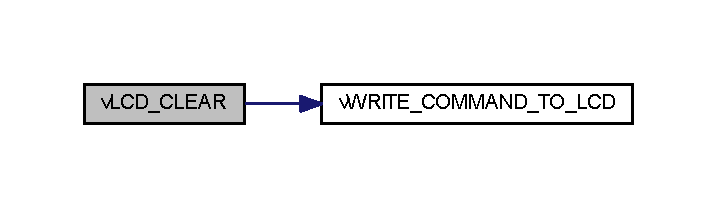
\includegraphics[width=344pt]{_lib___l_c_d_8c_af8b7dfeae5ba29704c45de38cce48d9a_cgraph}
\end{center}
\end{figure}


\hypertarget{_lib___l_c_d_8c_a3e2400a3341c31ace343ec46c1458285}{\index{Lib\-\_\-\-L\-C\-D.\-c@{Lib\-\_\-\-L\-C\-D.\-c}!v\-L\-C\-D\-\_\-\-C\-L\-E\-A\-R\-\_\-\-B\-O\-T\-T\-O\-M@{v\-L\-C\-D\-\_\-\-C\-L\-E\-A\-R\-\_\-\-B\-O\-T\-T\-O\-M}}
\index{v\-L\-C\-D\-\_\-\-C\-L\-E\-A\-R\-\_\-\-B\-O\-T\-T\-O\-M@{v\-L\-C\-D\-\_\-\-C\-L\-E\-A\-R\-\_\-\-B\-O\-T\-T\-O\-M}!Lib_LCD.c@{Lib\-\_\-\-L\-C\-D.\-c}}
\subsubsection[{v\-L\-C\-D\-\_\-\-C\-L\-E\-A\-R\-\_\-\-B\-O\-T\-T\-O\-M}]{\setlength{\rightskip}{0pt plus 5cm}v\-L\-C\-D\-\_\-\-C\-L\-E\-A\-R\-\_\-\-B\-O\-T\-T\-O\-M (
\begin{DoxyParamCaption}
\item[{void}]{}
\end{DoxyParamCaption}
)}}\label{_lib___l_c_d_8c_a3e2400a3341c31ace343ec46c1458285}


Function to clear the bottom line of the L\-C\-D Display. 





Calls the function to set the cursor to the home position of the bottom row, write 24 spaces as a string, then return to the home position of the bottom row.

\mbox{[}in\mbox{]} nothing

\begin{DoxyReturn}{Returns}
nothing
\end{DoxyReturn}
Modification History\-:

11/17/2013 -\/ Original Function 11/24/2013 -\/ Added code to function Call function to set cursor for bottom row's home position

Call function to write string of 24 spaces to clear the bottom row

Call function to set cursor for bottom row's home position 

Definition at line 400 of file Lib\-\_\-\-L\-C\-D.\-c.


\begin{DoxyCode}
401 \{
403     \hyperlink{_lib___l_c_d_8c_ae689772c0ccc0f690d05790f3a8cd89e}{vLCD\_HOME\_BOTTOM\_LINE}();
405     \hyperlink{_lib___l_c_d_8c_a4c4dec8455090f9fa00b2c5d1fbc2543}{vLCD\_WRITE\_STRING}(\textcolor{stringliteral}{"                        "});
407     \hyperlink{_lib___l_c_d_8c_ae689772c0ccc0f690d05790f3a8cd89e}{vLCD\_HOME\_BOTTOM\_LINE}();
408 \}
\end{DoxyCode}


Here is the call graph for this function\-:\nopagebreak
\begin{figure}[H]
\begin{center}
\leavevmode
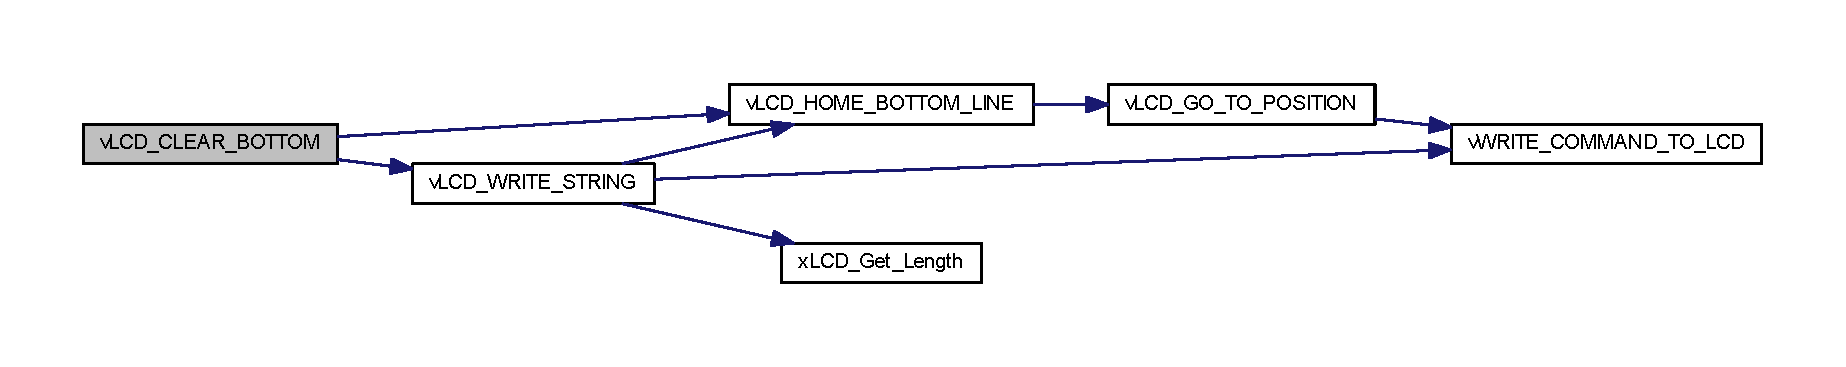
\includegraphics[width=350pt]{_lib___l_c_d_8c_a3e2400a3341c31ace343ec46c1458285_cgraph}
\end{center}
\end{figure}


\hypertarget{_lib___l_c_d_8c_a5d64774db98f8fa0c6d94565030064c1}{\index{Lib\-\_\-\-L\-C\-D.\-c@{Lib\-\_\-\-L\-C\-D.\-c}!v\-L\-C\-D\-\_\-\-C\-L\-E\-A\-R\-\_\-\-T\-O\-P@{v\-L\-C\-D\-\_\-\-C\-L\-E\-A\-R\-\_\-\-T\-O\-P}}
\index{v\-L\-C\-D\-\_\-\-C\-L\-E\-A\-R\-\_\-\-T\-O\-P@{v\-L\-C\-D\-\_\-\-C\-L\-E\-A\-R\-\_\-\-T\-O\-P}!Lib_LCD.c@{Lib\-\_\-\-L\-C\-D.\-c}}
\subsubsection[{v\-L\-C\-D\-\_\-\-C\-L\-E\-A\-R\-\_\-\-T\-O\-P}]{\setlength{\rightskip}{0pt plus 5cm}v\-L\-C\-D\-\_\-\-C\-L\-E\-A\-R\-\_\-\-T\-O\-P (
\begin{DoxyParamCaption}
\item[{void}]{}
\end{DoxyParamCaption}
)}}\label{_lib___l_c_d_8c_a5d64774db98f8fa0c6d94565030064c1}


Function to clear the top line of the L\-C\-D Display. 





Calls the function to set the cursor to the home position of the top row, write 24 spaces as a string, then return to the home position of the top row.

\mbox{[}in\mbox{]} nothing

\begin{DoxyReturn}{Returns}
nothing
\end{DoxyReturn}
Modification History\-:

11/17/2013 -\/ Original Function 11/24/2013 -\/ Added code to function Call function to set cursor for top row's home position

Call function to write string of 24 spaces to clear the top row

Call function to set cursor for top row's home position 

Definition at line 369 of file Lib\-\_\-\-L\-C\-D.\-c.


\begin{DoxyCode}
370 \{
372     \hyperlink{_lib___l_c_d_8c_a4427826e170410fece5aa9ff81f13d67}{vLCD\_HOME\_TOP\_LINE}();
374     \hyperlink{_lib___l_c_d_8c_a4c4dec8455090f9fa00b2c5d1fbc2543}{vLCD\_WRITE\_STRING}(\textcolor{stringliteral}{"                        "});
376     \hyperlink{_lib___l_c_d_8c_a4427826e170410fece5aa9ff81f13d67}{vLCD\_HOME\_TOP\_LINE}();
377 \}
\end{DoxyCode}


Here is the call graph for this function\-:\nopagebreak
\begin{figure}[H]
\begin{center}
\leavevmode
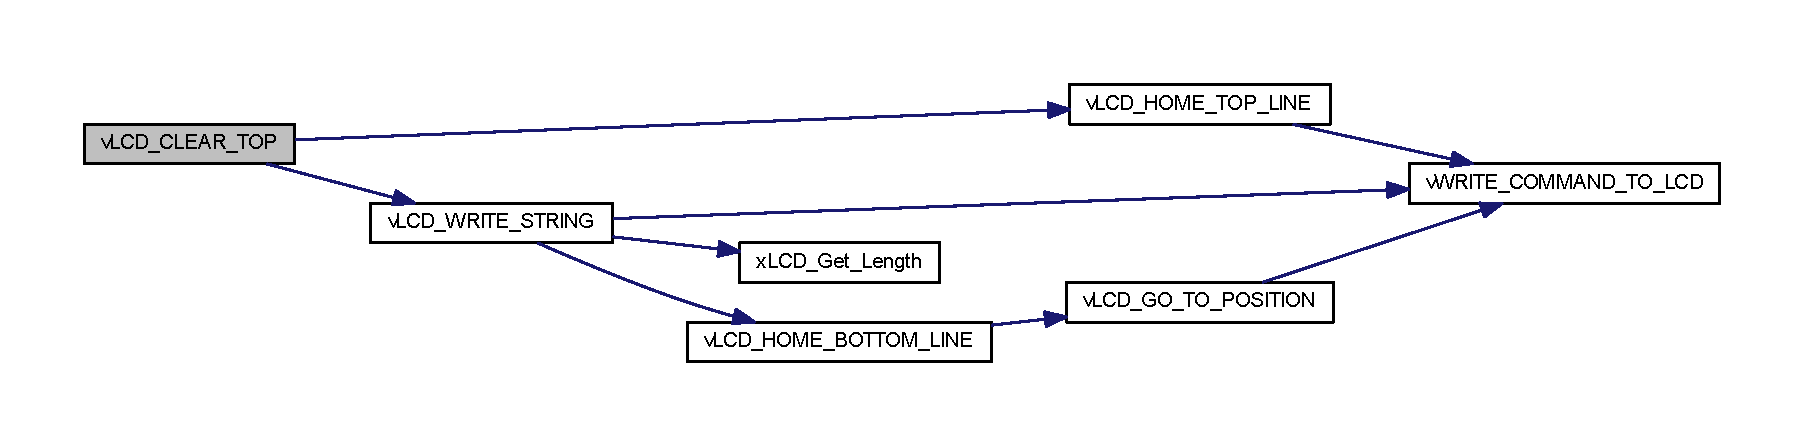
\includegraphics[width=350pt]{_lib___l_c_d_8c_a5d64774db98f8fa0c6d94565030064c1_cgraph}
\end{center}
\end{figure}


\hypertarget{_lib___l_c_d_8c_a3d78bee51edcb0ebe6cf4936147bb207}{\index{Lib\-\_\-\-L\-C\-D.\-c@{Lib\-\_\-\-L\-C\-D.\-c}!v\-L\-C\-D\-\_\-\-G\-O\-\_\-\-T\-O\-\_\-\-P\-O\-S\-I\-T\-I\-O\-N@{v\-L\-C\-D\-\_\-\-G\-O\-\_\-\-T\-O\-\_\-\-P\-O\-S\-I\-T\-I\-O\-N}}
\index{v\-L\-C\-D\-\_\-\-G\-O\-\_\-\-T\-O\-\_\-\-P\-O\-S\-I\-T\-I\-O\-N@{v\-L\-C\-D\-\_\-\-G\-O\-\_\-\-T\-O\-\_\-\-P\-O\-S\-I\-T\-I\-O\-N}!Lib_LCD.c@{Lib\-\_\-\-L\-C\-D.\-c}}
\subsubsection[{v\-L\-C\-D\-\_\-\-G\-O\-\_\-\-T\-O\-\_\-\-P\-O\-S\-I\-T\-I\-O\-N}]{\setlength{\rightskip}{0pt plus 5cm}void v\-L\-C\-D\-\_\-\-G\-O\-\_\-\-T\-O\-\_\-\-P\-O\-S\-I\-T\-I\-O\-N (
\begin{DoxyParamCaption}
\item[{uint8\-\_\-t}]{, }
\item[{uint8\-\_\-t}]{}
\end{DoxyParamCaption}
)}}\label{_lib___l_c_d_8c_a3d78bee51edcb0ebe6cf4936147bb207}
Function To go directly to a set of X,Y coordinates on the L\-C\-D 

Definition at line 523 of file Lib\-\_\-\-L\-C\-D.\-c.


\begin{DoxyCode}
524 \{
525     \textcolor{comment}{//save the current position}
526     \textcolor{keyword}{register} uint8\_t DDRAMAddr;
527     
528     \textcolor{comment}{// For each line o the LCD}
529     \textcolor{keywordflow}{switch}(y)
530     \{
531         \textcolor{keywordflow}{case} 0: 
532             \textcolor{comment}{//for the top line, set the DDRAM address }
533             \textcolor{comment}{//move a certain number of characters to the right}
534             DDRAMAddr = LCD\_LINE0\_DDRAMADDR + x;
535         \textcolor{keywordflow}{break};
536         
537         \textcolor{keywordflow}{case} 1: 
538             \textcolor{comment}{//for the bottom line, set the DDRAM address }
539             \textcolor{comment}{//move a certain number of characters to the right}
540             DDRAMAddr = LCD\_LINE1\_DDRAMADDR + x;
541         \textcolor{keywordflow}{break};
542         
543         \textcolor{keywordflow}{default}: 
544             \textcolor{comment}{//default to the top left of the LCD if nothing is specified}
545             DDRAMAddr = LCD\_LINE0\_DDRAMADDR+x;
546     \}
547     
548     \textcolor{comment}{//save current cursor position X}
549     \hyperlink{_lib___l_c_d_8h_af3836e0e465249949a42c1711a29b026}{CURSOR\_X\_POSITION} = x;
550     \textcolor{comment}{//save current cursor position Y}
551     \hyperlink{_lib___l_c_d_8h_aa8060b8676b9666d5b1357bb896a7cfa}{CURSOR\_Y\_POSITION} = y;
552     
553     \textcolor{comment}{// send a command to set the data address}
554     \hyperlink{_lib___l_c_d_8c_a03a66d0dc99ddbf838e4699cb1f0c568}{vWRITE\_COMMAND\_TO\_LCD}(INSTR\_WR, 1 <<LCD\_DDRAM | DDRAMAddr);
555 \}
\end{DoxyCode}


Here is the call graph for this function\-:\nopagebreak
\begin{figure}[H]
\begin{center}
\leavevmode
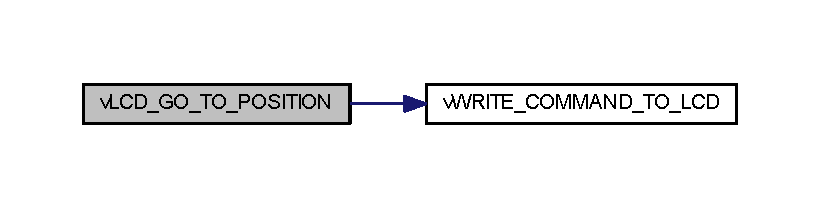
\includegraphics[width=350pt]{_lib___l_c_d_8c_a3d78bee51edcb0ebe6cf4936147bb207_cgraph}
\end{center}
\end{figure}




Here is the caller graph for this function\-:\nopagebreak
\begin{figure}[H]
\begin{center}
\leavevmode
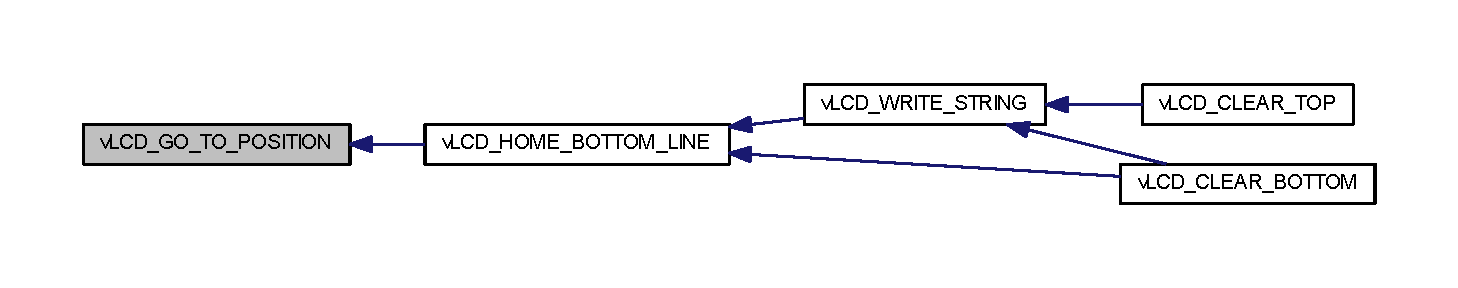
\includegraphics[width=350pt]{_lib___l_c_d_8c_a3d78bee51edcb0ebe6cf4936147bb207_icgraph}
\end{center}
\end{figure}


\hypertarget{_lib___l_c_d_8c_ae689772c0ccc0f690d05790f3a8cd89e}{\index{Lib\-\_\-\-L\-C\-D.\-c@{Lib\-\_\-\-L\-C\-D.\-c}!v\-L\-C\-D\-\_\-\-H\-O\-M\-E\-\_\-\-B\-O\-T\-T\-O\-M\-\_\-\-L\-I\-N\-E@{v\-L\-C\-D\-\_\-\-H\-O\-M\-E\-\_\-\-B\-O\-T\-T\-O\-M\-\_\-\-L\-I\-N\-E}}
\index{v\-L\-C\-D\-\_\-\-H\-O\-M\-E\-\_\-\-B\-O\-T\-T\-O\-M\-\_\-\-L\-I\-N\-E@{v\-L\-C\-D\-\_\-\-H\-O\-M\-E\-\_\-\-B\-O\-T\-T\-O\-M\-\_\-\-L\-I\-N\-E}!Lib_LCD.c@{Lib\-\_\-\-L\-C\-D.\-c}}
\subsubsection[{v\-L\-C\-D\-\_\-\-H\-O\-M\-E\-\_\-\-B\-O\-T\-T\-O\-M\-\_\-\-L\-I\-N\-E}]{\setlength{\rightskip}{0pt plus 5cm}v\-L\-C\-D\-\_\-\-H\-O\-M\-E\-\_\-\-B\-O\-T\-T\-O\-M\-\_\-\-L\-I\-N\-E (
\begin{DoxyParamCaption}
\item[{void}]{}
\end{DoxyParamCaption}
)}}\label{_lib___l_c_d_8c_ae689772c0ccc0f690d05790f3a8cd89e}


Function to return to home position on the bottom line of the L\-C\-D. 





Function is called to return the cursor to the first position on the bottom line of the L\-C\-D.

This allows for the the bottom line to be ready to write independently from the top line.

\mbox{[}in\mbox{]} none

\begin{DoxyReturn}{Returns}
nothing
\end{DoxyReturn}
Modification History\-:

11/15/2013 -\/ Original Function 

Definition at line 607 of file Lib\-\_\-\-L\-C\-D.\-c.


\begin{DoxyCode}
608 \{
609     \textcolor{comment}{//move the cursor to the bottom left position on the LCD}
610     \hyperlink{_lib___l_c_d_8c_a3d78bee51edcb0ebe6cf4936147bb207}{vLCD\_GO\_TO\_POSITION}(0,1);
611 \}
\end{DoxyCode}


Here is the call graph for this function\-:\nopagebreak
\begin{figure}[H]
\begin{center}
\leavevmode
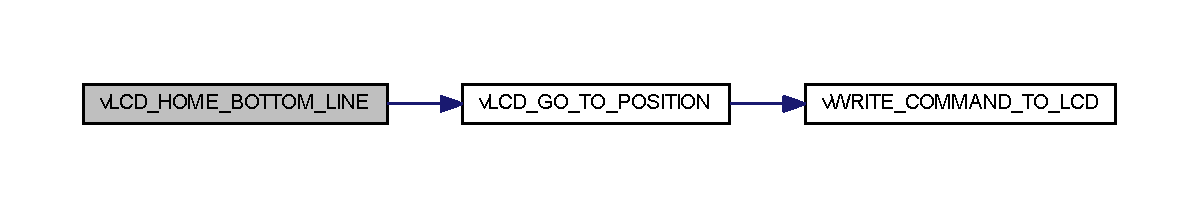
\includegraphics[width=350pt]{_lib___l_c_d_8c_ae689772c0ccc0f690d05790f3a8cd89e_cgraph}
\end{center}
\end{figure}




Here is the caller graph for this function\-:\nopagebreak
\begin{figure}[H]
\begin{center}
\leavevmode
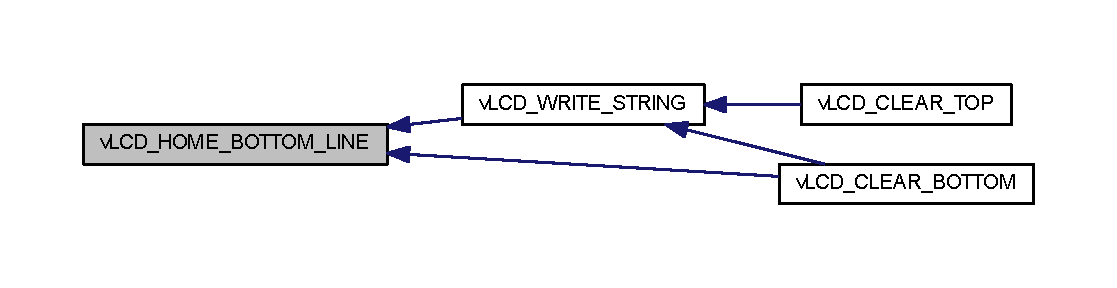
\includegraphics[width=350pt]{_lib___l_c_d_8c_ae689772c0ccc0f690d05790f3a8cd89e_icgraph}
\end{center}
\end{figure}


\hypertarget{_lib___l_c_d_8c_a4427826e170410fece5aa9ff81f13d67}{\index{Lib\-\_\-\-L\-C\-D.\-c@{Lib\-\_\-\-L\-C\-D.\-c}!v\-L\-C\-D\-\_\-\-H\-O\-M\-E\-\_\-\-T\-O\-P\-\_\-\-L\-I\-N\-E@{v\-L\-C\-D\-\_\-\-H\-O\-M\-E\-\_\-\-T\-O\-P\-\_\-\-L\-I\-N\-E}}
\index{v\-L\-C\-D\-\_\-\-H\-O\-M\-E\-\_\-\-T\-O\-P\-\_\-\-L\-I\-N\-E@{v\-L\-C\-D\-\_\-\-H\-O\-M\-E\-\_\-\-T\-O\-P\-\_\-\-L\-I\-N\-E}!Lib_LCD.c@{Lib\-\_\-\-L\-C\-D.\-c}}
\subsubsection[{v\-L\-C\-D\-\_\-\-H\-O\-M\-E\-\_\-\-T\-O\-P\-\_\-\-L\-I\-N\-E}]{\setlength{\rightskip}{0pt plus 5cm}v\-L\-C\-D\-\_\-\-H\-O\-M\-E\-\_\-\-T\-O\-P\-\_\-\-L\-I\-N\-E (
\begin{DoxyParamCaption}
\item[{void}]{}
\end{DoxyParamCaption}
)}}\label{_lib___l_c_d_8c_a4427826e170410fece5aa9ff81f13d67}


Function to return to home position on the top line of the L\-C\-D. 





Function is called to return the cursor to the first position on the top line of the L\-C\-D.

This allows for the the top line to be ready to write independently from the bottom line.

\mbox{[}in\mbox{]} none

\begin{DoxyReturn}{Returns}
nothing
\end{DoxyReturn}
Modification History\-:

11/15/2013 -\/ Original Function 

Definition at line 579 of file Lib\-\_\-\-L\-C\-D.\-c.


\begin{DoxyCode}
580 \{
581     \textcolor{comment}{//move cursor to the top left position of the LCD}
582     \hyperlink{_lib___l_c_d_8c_a03a66d0dc99ddbf838e4699cb1f0c568}{vWRITE\_COMMAND\_TO\_LCD}(INSTR\_WR, 1 << \hyperlink{_lib___l_c_d_8h_a207e17a2f807f034c0fc055010928a16}{LCD\_HOME\_TOP\_LINE});
583 \}
\end{DoxyCode}


Here is the call graph for this function\-:\nopagebreak
\begin{figure}[H]
\begin{center}
\leavevmode
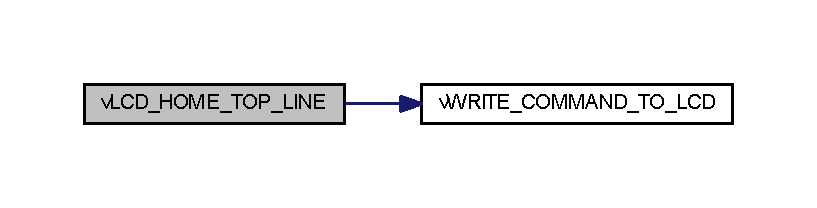
\includegraphics[width=350pt]{_lib___l_c_d_8c_a4427826e170410fece5aa9ff81f13d67_cgraph}
\end{center}
\end{figure}




Here is the caller graph for this function\-:\nopagebreak
\begin{figure}[H]
\begin{center}
\leavevmode
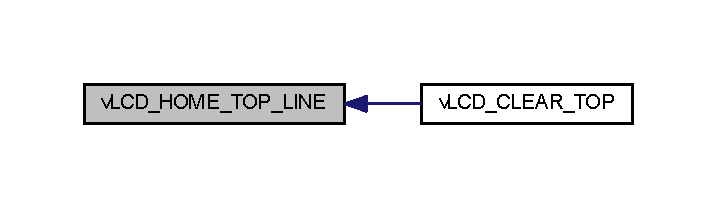
\includegraphics[width=344pt]{_lib___l_c_d_8c_a4427826e170410fece5aa9ff81f13d67_icgraph}
\end{center}
\end{figure}


\hypertarget{_lib___l_c_d_8c_a801b1b8096ae349442402ff4260357e8}{\index{Lib\-\_\-\-L\-C\-D.\-c@{Lib\-\_\-\-L\-C\-D.\-c}!v\-L\-C\-D\-\_\-\-I\-N\-I\-T\-I\-A\-L\-I\-Z\-A\-T\-I\-O\-N@{v\-L\-C\-D\-\_\-\-I\-N\-I\-T\-I\-A\-L\-I\-Z\-A\-T\-I\-O\-N}}
\index{v\-L\-C\-D\-\_\-\-I\-N\-I\-T\-I\-A\-L\-I\-Z\-A\-T\-I\-O\-N@{v\-L\-C\-D\-\_\-\-I\-N\-I\-T\-I\-A\-L\-I\-Z\-A\-T\-I\-O\-N}!Lib_LCD.c@{Lib\-\_\-\-L\-C\-D.\-c}}
\subsubsection[{v\-L\-C\-D\-\_\-\-I\-N\-I\-T\-I\-A\-L\-I\-Z\-A\-T\-I\-O\-N}]{\setlength{\rightskip}{0pt plus 5cm}v\-L\-C\-D\-\_\-\-I\-N\-I\-T\-I\-A\-L\-I\-Z\-A\-T\-I\-O\-N (
\begin{DoxyParamCaption}
\item[{void}]{}
\end{DoxyParamCaption}
)}}\label{_lib___l_c_d_8c_a801b1b8096ae349442402ff4260357e8}


Function to initialize the L\-D\-C. 





Function is called to initialize the L\-C\-D into either 4 bit or 8 bit mode off of the flowcharts on pages 26 and 27 of the K\-S6600\-U datasheet

\mbox{[}in\mbox{]} none

\begin{DoxyReturn}{Returns}
nothing
\end{DoxyReturn}
Modification History\-:

11/17/2013 -\/ Original Function 

Definition at line 48 of file Lib\-\_\-\-L\-C\-D.\-c.


\begin{DoxyCode}
49 \{
50     \textcolor{keywordtype}{unsigned} \textcolor{keywordtype}{char} Instructions = 0x00;
51     
52 \textcolor{preprocessor}{    #ifdef BITMODE4}
53 \textcolor{preprocessor}{}
54         \_delay\_ms(35);
55         
56         \textcolor{comment}{/***************************************************************************/}
65         Instructions = (1<<\hyperlink{_lib___l_c_d_8h_a5b91fe480c768d4f246f3890207bfbfc}{LCD\_D5});
66         
67         \hyperlink{_lib___l_c_d_8c_a03a66d0dc99ddbf838e4699cb1f0c568}{vWRITE\_COMMAND\_TO\_LCD}(INSTR\_WR, Instructions);
68         \hyperlink{_lib___l_c_d_8c_a03a66d0dc99ddbf838e4699cb1f0c568}{vWRITE\_COMMAND\_TO\_LCD}(INSTR\_WR, Instructions);
69         
70         Instructions = (TWO\_LINE\_MODE<<\hyperlink{_lib___l_c_d_8h_abd65075e01c7413419581aedee5bcc24}{LCD\_D7})|(DISPLAY\_ON<<\hyperlink{_lib___l_c_d_8h_a72e105fcda5fd1c07b5f391379a439d4}{LCD\_D6});
71         
72         \hyperlink{_lib___l_c_d_8c_a03a66d0dc99ddbf838e4699cb1f0c568}{vWRITE\_COMMAND\_TO\_LCD}(INSTR\_WR, Instructions);
73         
75         \_delay\_us(50);
76         
77         \textcolor{comment}{/***************************************************************************/}
87         Instructions = 0x00;
88         
89         \hyperlink{_lib___l_c_d_8c_a03a66d0dc99ddbf838e4699cb1f0c568}{vWRITE\_COMMAND\_TO\_LCD}(INSTR\_WR, Instructions);
90         
91         Instructions = (1 << \hyperlink{_lib___l_c_d_8h_abd65075e01c7413419581aedee5bcc24}{LCD\_D7}) | 
92               (DISPLAY\_ON << \hyperlink{_lib___l_c_d_8h_a72e105fcda5fd1c07b5f391379a439d4}{LCD\_D6}) | 
93                (CURSOR\_ON << \hyperlink{_lib___l_c_d_8h_a5b91fe480c768d4f246f3890207bfbfc}{LCD\_D5}) | 
94          (CURSOR\_BLINK\_ON << \hyperlink{_lib___l_c_d_8h_ade7e247311032a474711416da480ed8b}{LCD\_D4}));
95          
96          \hyperlink{_lib___l_c_d_8c_a03a66d0dc99ddbf838e4699cb1f0c568}{vWRITE\_COMMAND\_TO\_LCD}(INSTR\_WR, Instructions);
97          
99         \_delay\_us(50);
100         
101         \textcolor{comment}{/***************************************************************************/}
105         Instructions = 0x00;
106         
107         \hyperlink{_lib___l_c_d_8c_a03a66d0dc99ddbf838e4699cb1f0c568}{vWRITE\_COMMAND\_TO\_LCD}(INSTR\_WR, Instructions);
108         
111         Instructions = (1<<\hyperlink{_lib___l_c_d_8h_ade7e247311032a474711416da480ed8b}{LCD\_D4});
112         
113         \hyperlink{_lib___l_c_d_8c_a03a66d0dc99ddbf838e4699cb1f0c568}{vWRITE\_COMMAND\_TO\_LCD}(INSTR\_WR, Instructions);
114         
116         \_delay\_us(1600);
117         
118         \textcolor{comment}{/***************************************************************************/}
122         Instructions = 0x00;
123         
124         \hyperlink{_lib___l_c_d_8c_a03a66d0dc99ddbf838e4699cb1f0c568}{vWRITE\_COMMAND\_TO\_LCD}(INSTR\_WR, Instructions);
125         
131         Instructions =  (1 << \hyperlink{_lib___l_c_d_8h_a72e105fcda5fd1c07b5f391379a439d4}{LCD\_D6}) | 
132            (INCREMENT\_MODE << \hyperlink{_lib___l_c_d_8h_a5b91fe480c768d4f246f3890207bfbfc}{LCD\_D5}) | 
133         (ENTIRE\_SHIFT\_MODE << \hyperlink{_lib___l_c_d_8h_ade7e247311032a474711416da480ed8b}{LCD\_D4});
134         
135         \hyperlink{_lib___l_c_d_8c_a03a66d0dc99ddbf838e4699cb1f0c568}{vWRITE\_COMMAND\_TO\_LCD}(INSTR\_WR, Instructions);
136 \textcolor{preprocessor}{    #endif;}
137 \textcolor{preprocessor}{}    
138 \textcolor{preprocessor}{    #ifdef BITMODE8}
139 \textcolor{preprocessor}{}    
141         \_delay\_ms(35);
142         
143         \textcolor{comment}{/***************************************************************************/}
152         Instructions = (1 << \hyperlink{_lib___l_c_d_8h_a5b91fe480c768d4f246f3890207bfbfc}{LCD\_D5}) |
153                        (1 << \hyperlink{_lib___l_c_d_8h_ade7e247311032a474711416da480ed8b}{LCD\_D4}) | 
154            (TWO\_LINE\_MODE << \hyperlink{_lib___l_c_d_8h_a3d23f1f20ad1f0fb190f4a10334f4bf1}{LCD\_D3}) | 
155               (DISPLAY\_ON << \hyperlink{_lib___l_c_d_8h_aa97ea257a9007a9055e5f77e1b3336e5}{LCD\_D2}); 
156               
157         \hyperlink{_lib___l_c_d_8c_a03a66d0dc99ddbf838e4699cb1f0c568}{vWRITE\_COMMAND\_TO\_LCD}(INSTR\_WR, Instructions);
158                 
160         \_delay\_us(50);
161         
162         \textcolor{comment}{/***************************************************************************/}
172         Instructions = (1 << \hyperlink{_lib___l_c_d_8h_a3d23f1f20ad1f0fb190f4a10334f4bf1}{LCD\_D3}) | 
173               (DISPLAY\_ON << \hyperlink{_lib___l_c_d_8h_aa97ea257a9007a9055e5f77e1b3336e5}{LCD\_D2}) | 
174                (CURSOR\_ON << \hyperlink{_lib___l_c_d_8h_ac6b74016e58d58b47230a2d0aaf959d8}{LCD\_D1}) | 
175          (CURSOR\_BLINK\_ON << 0);
176          
177          \hyperlink{_lib___l_c_d_8c_a03a66d0dc99ddbf838e4699cb1f0c568}{vWRITE\_COMMAND\_TO\_LCD}(INSTR\_WR, Instructions);
178          
180         \_delay\_us(50);
181         
182         \textcolor{comment}{/***************************************************************************/}
188         Instructions = 0x01;
189         
190         \hyperlink{_lib___l_c_d_8c_a03a66d0dc99ddbf838e4699cb1f0c568}{vWRITE\_COMMAND\_TO\_LCD}(INSTR\_WR, Instructions);
191         
193         \_delay\_us(1600);
194         
195         \textcolor{comment}{/***************************************************************************/}
204         Instructions =  (1 << \hyperlink{_lib___l_c_d_8h_aa97ea257a9007a9055e5f77e1b3336e5}{LCD\_D2}) | 
205            (INCREMENT\_MODE << \hyperlink{_lib___l_c_d_8h_ac6b74016e58d58b47230a2d0aaf959d8}{LCD\_D1}) | 
206         (ENTIRE\_SHIFT\_MODE << 0);
207         
208         \hyperlink{_lib___l_c_d_8c_a03a66d0dc99ddbf838e4699cb1f0c568}{vWRITE\_COMMAND\_TO\_LCD}(INSTR\_WR, Instructions);
209         
210 \textcolor{preprocessor}{    #endif;}
211 \textcolor{preprocessor}{}    
212 \}
\end{DoxyCode}


Here is the call graph for this function\-:\nopagebreak
\begin{figure}[H]
\begin{center}
\leavevmode
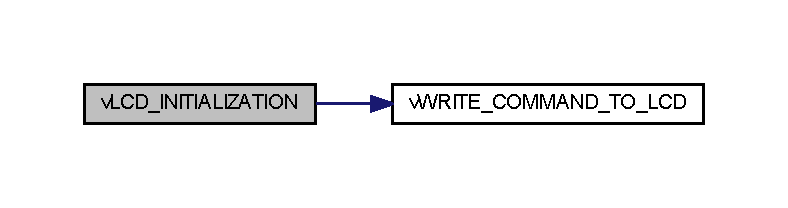
\includegraphics[width=350pt]{_lib___l_c_d_8c_a801b1b8096ae349442402ff4260357e8_cgraph}
\end{center}
\end{figure}


\hypertarget{_lib___l_c_d_8c_afd6340508e9e341f1a8c7ba4228e27f9}{\index{Lib\-\_\-\-L\-C\-D.\-c@{Lib\-\_\-\-L\-C\-D.\-c}!v\-L\-C\-D\-\_\-\-O\-N\-\_\-\-O\-F\-F@{v\-L\-C\-D\-\_\-\-O\-N\-\_\-\-O\-F\-F}}
\index{v\-L\-C\-D\-\_\-\-O\-N\-\_\-\-O\-F\-F@{v\-L\-C\-D\-\_\-\-O\-N\-\_\-\-O\-F\-F}!Lib_LCD.c@{Lib\-\_\-\-L\-C\-D.\-c}}
\subsubsection[{v\-L\-C\-D\-\_\-\-O\-N\-\_\-\-O\-F\-F}]{\setlength{\rightskip}{0pt plus 5cm}v\-L\-C\-D\-\_\-\-O\-N\-\_\-\-O\-F\-F (
\begin{DoxyParamCaption}
\item[{void}]{}
\end{DoxyParamCaption}
)}}\label{_lib___l_c_d_8c_afd6340508e9e341f1a8c7ba4228e27f9}


Function to toggle L\-C\-D on and off. 





Checks the current status of the L\-C\-D. If the L\-C\-D is on, toggle it so it's off. If the L\-C\-D is off, turn it on. Uses the v\-L\-C\-D\-\_\-\-W\-R\-I\-T\-E command to send instructions to the L\-C\-D.

\mbox{[}in\mbox{]} nothing

\begin{DoxyReturn}{Returns}
nothing
\end{DoxyReturn}
Modification History\-:

11/18/2013 -\/ Original Function 11/24/2013 -\/ Added code to function Create command to toggle L\-C\-D Display

Toggle the On\-Off\-Status tracker variable

Toggle L\-C\-D 

Definition at line 431 of file Lib\-\_\-\-L\-C\-D.\-c.


\begin{DoxyCode}
432 \{
434     uint8\_t LCD\_Command = 
435         (1 << \hyperlink{_lib___l_c_d_8h_aa57a26c661193bfb41377f080d15b4d6}{LCD\_ON\_OFF\_INSTRCUTION}) |
436         (\hyperlink{_lib___l_c_d_8h_a7306354fa1b76399437e38800816c915}{OnOffStatus} << LCD\_ON\_INSTRUCTION) |
437         (\hyperlink{_lib___l_c_d_8h_aaa9d50b1d874e351a1bafc33f7f8b22d}{configCURSOR\_SHOW} << LCD\_CURSOR\_SHOW\_INSTRUCTION) |
438         (configCURSOR\_BLINK << LCD\_CURSOR\_BLINK\_INSTRUCTION);
439     
441     \hyperlink{_lib___l_c_d_8h_a7306354fa1b76399437e38800816c915}{OnOffStatus} = \hyperlink{_lib___l_c_d_8h_a7306354fa1b76399437e38800816c915}{OnOffStatus} ^ 0x01;
442     
444     \hyperlink{_lib___l_c_d_8c_a03a66d0dc99ddbf838e4699cb1f0c568}{vWRITE\_COMMAND\_TO\_LCD}(0, LCD\_Command);
445 \}
\end{DoxyCode}


Here is the call graph for this function\-:\nopagebreak
\begin{figure}[H]
\begin{center}
\leavevmode
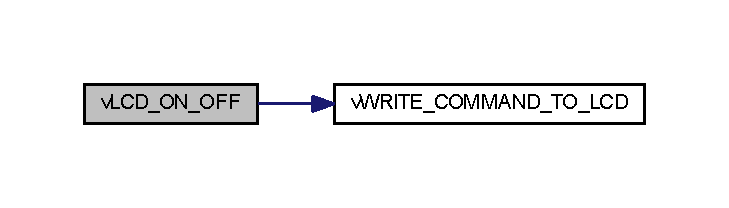
\includegraphics[width=350pt]{_lib___l_c_d_8c_afd6340508e9e341f1a8c7ba4228e27f9_cgraph}
\end{center}
\end{figure}


\hypertarget{_lib___l_c_d_8c_a4c4dec8455090f9fa00b2c5d1fbc2543}{\index{Lib\-\_\-\-L\-C\-D.\-c@{Lib\-\_\-\-L\-C\-D.\-c}!v\-L\-C\-D\-\_\-\-W\-R\-I\-T\-E\-\_\-\-S\-T\-R\-I\-N\-G@{v\-L\-C\-D\-\_\-\-W\-R\-I\-T\-E\-\_\-\-S\-T\-R\-I\-N\-G}}
\index{v\-L\-C\-D\-\_\-\-W\-R\-I\-T\-E\-\_\-\-S\-T\-R\-I\-N\-G@{v\-L\-C\-D\-\_\-\-W\-R\-I\-T\-E\-\_\-\-S\-T\-R\-I\-N\-G}!Lib_LCD.c@{Lib\-\_\-\-L\-C\-D.\-c}}
\subsubsection[{v\-L\-C\-D\-\_\-\-W\-R\-I\-T\-E\-\_\-\-S\-T\-R\-I\-N\-G}]{\setlength{\rightskip}{0pt plus 5cm}v\-L\-C\-D\-\_\-\-W\-R\-I\-T\-E\-\_\-\-S\-T\-R\-I\-N\-G (
\begin{DoxyParamCaption}
\item[{char $\ast$}]{str\-\_\-ptr}
\end{DoxyParamCaption}
)}}\label{_lib___l_c_d_8c_a4c4dec8455090f9fa00b2c5d1fbc2543}


Function to write strings to the L\-C\-D. 





Function is used to take in a string of characters and display the string to the L\-C\-D

\mbox{[}in\mbox{]} $\ast$str\-\_\-ptr

\begin{DoxyReturn}{Returns}
nothing
\end{DoxyReturn}
Modification History\-:

11/17/2013 -\/ Original Function 11/23/2013 -\/ Addec Code If text wrap is enabled 

Definition at line 295 of file Lib\-\_\-\-L\-C\-D.\-c.


\begin{DoxyCode}
296 \{   
297     \textcolor{keywordflow}{while}(*str\_ptr != \textcolor{charliteral}{'\(\backslash\)0'})     \textcolor{comment}{//move through the string until the end is reached}
298     \{
300 \textcolor{preprocessor}{        #ifdef configTEXT\_WRAP}
301 \textcolor{preprocessor}{}\textcolor{preprocessor}{            #if configTEXT\_WRAP == 1}
302 \textcolor{preprocessor}{}        
304                 \textcolor{keywordflow}{if}( \hyperlink{_lib___l_c_d_8c_a1d0d7788aeded6a84e4149f2351beaf8}{xLCD\_Get\_Length}()== 24)
305                     \hyperlink{_lib___l_c_d_8c_ae689772c0ccc0f690d05790f3a8cd89e}{vLCD\_HOME\_BOTTOM\_LINE}(); \textcolor{comment}{//Continue on to the bottom line}
306         
307 \textcolor{preprocessor}{            #endif}
308 \textcolor{preprocessor}{}\textcolor{preprocessor}{        #endif}
309 \textcolor{preprocessor}{}        \hyperlink{_lib___l_c_d_8c_a03a66d0dc99ddbf838e4699cb1f0c568}{vWRITE\_COMMAND\_TO\_LCD}(DATA\_WR, *str\_ptr++);
310     \}   
311 \}
\end{DoxyCode}


Here is the call graph for this function\-:\nopagebreak
\begin{figure}[H]
\begin{center}
\leavevmode
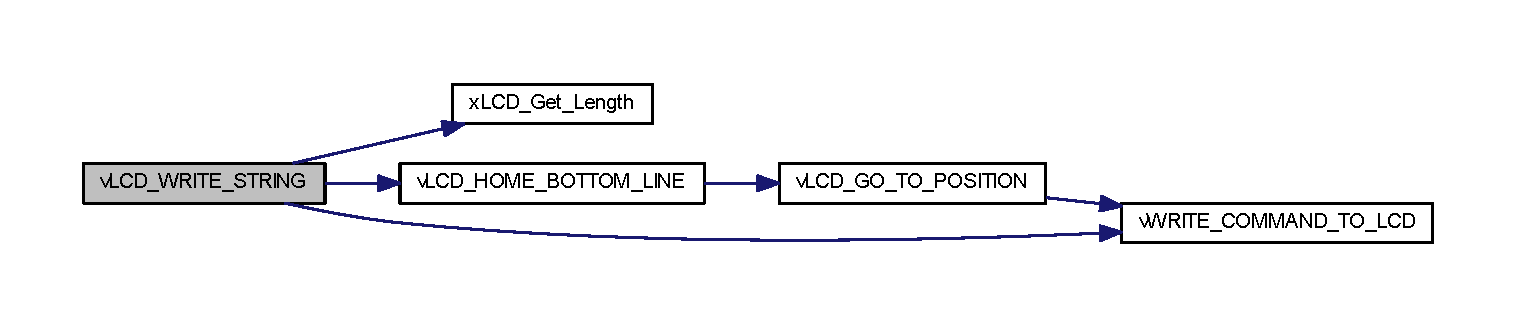
\includegraphics[width=350pt]{_lib___l_c_d_8c_a4c4dec8455090f9fa00b2c5d1fbc2543_cgraph}
\end{center}
\end{figure}




Here is the caller graph for this function\-:\nopagebreak
\begin{figure}[H]
\begin{center}
\leavevmode
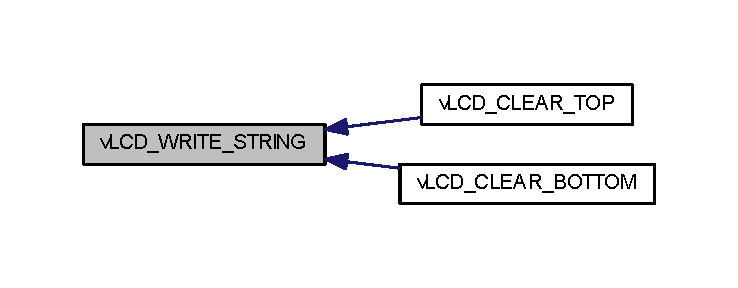
\includegraphics[width=350pt]{_lib___l_c_d_8c_a4c4dec8455090f9fa00b2c5d1fbc2543_icgraph}
\end{center}
\end{figure}


\hypertarget{_lib___l_c_d_8c_a03a66d0dc99ddbf838e4699cb1f0c568}{\index{Lib\-\_\-\-L\-C\-D.\-c@{Lib\-\_\-\-L\-C\-D.\-c}!v\-W\-R\-I\-T\-E\-\_\-\-C\-O\-M\-M\-A\-N\-D\-\_\-\-T\-O\-\_\-\-L\-C\-D@{v\-W\-R\-I\-T\-E\-\_\-\-C\-O\-M\-M\-A\-N\-D\-\_\-\-T\-O\-\_\-\-L\-C\-D}}
\index{v\-W\-R\-I\-T\-E\-\_\-\-C\-O\-M\-M\-A\-N\-D\-\_\-\-T\-O\-\_\-\-L\-C\-D@{v\-W\-R\-I\-T\-E\-\_\-\-C\-O\-M\-M\-A\-N\-D\-\_\-\-T\-O\-\_\-\-L\-C\-D}!Lib_LCD.c@{Lib\-\_\-\-L\-C\-D.\-c}}
\subsubsection[{v\-W\-R\-I\-T\-E\-\_\-\-C\-O\-M\-M\-A\-N\-D\-\_\-\-T\-O\-\_\-\-L\-C\-D}]{\setlength{\rightskip}{0pt plus 5cm}void v\-W\-R\-I\-T\-E\-\_\-\-C\-O\-M\-M\-A\-N\-D\-\_\-\-T\-O\-\_\-\-L\-C\-D (
\begin{DoxyParamCaption}
\item[{char}]{R\-S, }
\item[{char}]{data}
\end{DoxyParamCaption}
)}}\label{_lib___l_c_d_8c_a03a66d0dc99ddbf838e4699cb1f0c568}
Function to Write commands to an L\-C\-D Set Read/\-Write High

Set D\-B7 pin to read

Wait for Busy flag to clear

Set L\-C\-D\-\_\-\-D7 pin for output

Enable display for use

Wait for Busy flag to clear 

Definition at line 238 of file Lib\-\_\-\-L\-C\-D.\-c.


\begin{DoxyCode}
239 \{
240     \textcolor{keywordflow}{if}(RS == DATA\_WR) \hyperlink{_lib___l_c_d_8h_a488115f911c9dcfb0bad83c6b0912965}{LCP} = 1<<\hyperlink{_lib___l_c_d_8h_a4781e073871c6f27f89b9463ad3a4ed1}{LCD\_RS}; \textcolor{comment}{/*Set RS high to write data*/} 
241     \textcolor{keywordflow}{else} \hyperlink{_lib___l_c_d_8h_a488115f911c9dcfb0bad83c6b0912965}{LCP} = 0x00; \textcolor{comment}{/*Set RS low to write instructions*/}
242     
244     \hyperlink{_lib___l_c_d_8h_a488115f911c9dcfb0bad83c6b0912965}{LCP} = \hyperlink{_lib___l_c_d_8h_a488115f911c9dcfb0bad83c6b0912965}{LCP} | 1<<\hyperlink{_lib___l_c_d_8h_a26089a10ddd59a0dc7283c19ccc02533}{LCD\_RW}; 
245 
247     \hyperlink{_lib___l_c_d_8h_a8a47e7956b4dd0e990db51cd70d9eac8}{LDDR} = \hyperlink{_lib___l_c_d_8h_a8a47e7956b4dd0e990db51cd70d9eac8}{LDDR} & 0x7F;
248     
250     \textcolor{keywordflow}{while}(\hyperlink{_lib___l_c_d_8h_a88979bbbc6cd7d8c557867826d755c1b}{LDP} & 0x80);
251     
253     \hyperlink{_lib___l_c_d_8h_a8a47e7956b4dd0e990db51cd70d9eac8}{LDDR} = \hyperlink{_lib___l_c_d_8h_a8a47e7956b4dd0e990db51cd70d9eac8}{LDDR} | (1 << \hyperlink{_lib___l_c_d_8h_abd65075e01c7413419581aedee5bcc24}{LCD\_D7});
254     
255     \textcolor{keywordflow}{if}(RS == DATA\_WR) \hyperlink{_lib___l_c_d_8h_a488115f911c9dcfb0bad83c6b0912965}{LCP} = 1 << \hyperlink{_lib___l_c_d_8h_a4781e073871c6f27f89b9463ad3a4ed1}{LCD\_RS};   \textcolor{comment}{/*Set RS high to write data*/} 
256     \textcolor{keywordflow}{else} \hyperlink{_lib___l_c_d_8h_a488115f911c9dcfb0bad83c6b0912965}{LCP} = 0x00; \textcolor{comment}{/*Set RS low to write instructions*/}
257     
259     \hyperlink{_lib___l_c_d_8h_a488115f911c9dcfb0bad83c6b0912965}{LCP} = \hyperlink{_lib___l_c_d_8h_a488115f911c9dcfb0bad83c6b0912965}{LCP} | 1<<\hyperlink{_lib___l_c_d_8h_a6ec15b1e813d1f56d2eb644a127e5d49}{LCD\_E}; 
260     
261     \textcolor{comment}{/* Write Data*/}
262     \hyperlink{_lib___l_c_d_8h_a88979bbbc6cd7d8c557867826d755c1b}{LDP} = data;
263     
265     \textcolor{keywordflow}{while}(\hyperlink{_lib___l_c_d_8h_a88979bbbc6cd7d8c557867826d755c1b}{LDP} & 0x80); 
266     
267     \textcolor{comment}{/*Set Read/Write low*/}
268     \hyperlink{_lib___l_c_d_8h_a488115f911c9dcfb0bad83c6b0912965}{LCP} = \hyperlink{_lib___l_c_d_8h_a488115f911c9dcfb0bad83c6b0912965}{LCP} & 1<<\hyperlink{_lib___l_c_d_8h_a4781e073871c6f27f89b9463ad3a4ed1}{LCD\_RS};
269     
270     \textcolor{comment}{/*Delay for at least 50us*/}
271     \_delay\_us(50);
272 \}
\end{DoxyCode}


Here is the caller graph for this function\-:\nopagebreak
\begin{figure}[H]
\begin{center}
\leavevmode
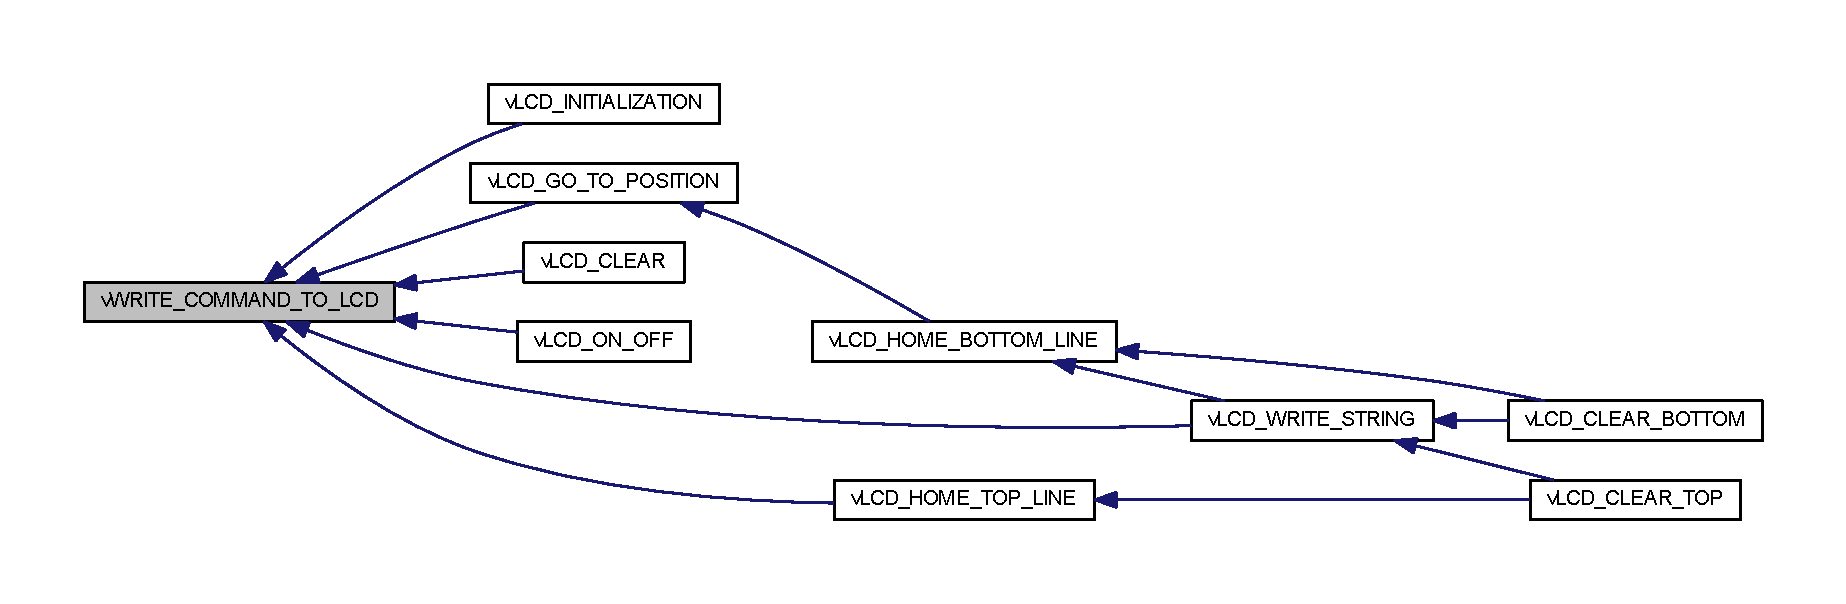
\includegraphics[width=350pt]{_lib___l_c_d_8c_a03a66d0dc99ddbf838e4699cb1f0c568_icgraph}
\end{center}
\end{figure}


\hypertarget{_lib___l_c_d_8c_a1d0d7788aeded6a84e4149f2351beaf8}{\index{Lib\-\_\-\-L\-C\-D.\-c@{Lib\-\_\-\-L\-C\-D.\-c}!x\-L\-C\-D\-\_\-\-Get\-\_\-\-Length@{x\-L\-C\-D\-\_\-\-Get\-\_\-\-Length}}
\index{x\-L\-C\-D\-\_\-\-Get\-\_\-\-Length@{x\-L\-C\-D\-\_\-\-Get\-\_\-\-Length}!Lib_LCD.c@{Lib\-\_\-\-L\-C\-D.\-c}}
\subsubsection[{x\-L\-C\-D\-\_\-\-Get\-\_\-\-Length}]{\setlength{\rightskip}{0pt plus 5cm}uint8\-\_\-t x\-L\-C\-D\-\_\-\-Get\-\_\-\-Length (
\begin{DoxyParamCaption}
{}
\end{DoxyParamCaption}
)}}\label{_lib___l_c_d_8c_a1d0d7788aeded6a84e4149f2351beaf8}
Function to track remaining characters on the L\-C\-D If the cursor is on the top line

give total available characters(top and bottom line)

If the cursor is on the bottom line

Give remaining characters available. 

Definition at line 475 of file Lib\-\_\-\-L\-C\-D.\-c.


\begin{DoxyCode}
476 \{
477     \textcolor{keywordflow}{switch}(\hyperlink{_lib___l_c_d_8h_aa8060b8676b9666d5b1357bb896a7cfa}{CURSOR\_Y\_POSITION})
478     \{
480         \textcolor{keywordflow}{case} 0:
482             \textcolor{keywordflow}{return} 48 - \hyperlink{_lib___l_c_d_8h_af3836e0e465249949a42c1711a29b026}{CURSOR\_X\_POSITION}; 
483             \textcolor{keywordflow}{break};
484             
486         \textcolor{keywordflow}{case} 1:
488             \textcolor{keywordflow}{return} 24 - \hyperlink{_lib___l_c_d_8h_af3836e0e465249949a42c1711a29b026}{CURSOR\_X\_POSITION}; 
489     \}
490 \}
\end{DoxyCode}


Here is the caller graph for this function\-:\nopagebreak
\begin{figure}[H]
\begin{center}
\leavevmode
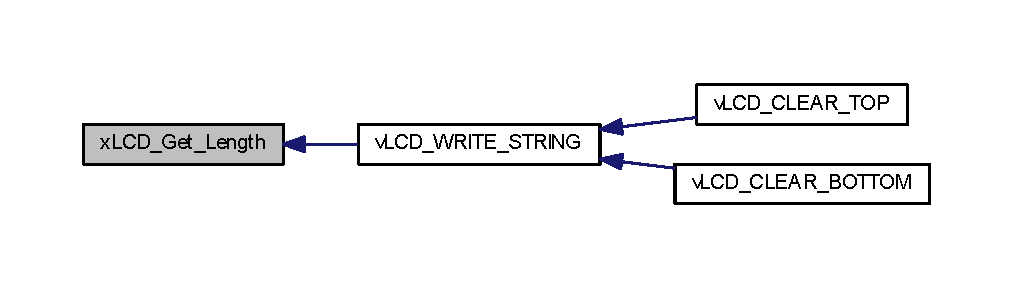
\includegraphics[width=350pt]{_lib___l_c_d_8c_a1d0d7788aeded6a84e4149f2351beaf8_icgraph}
\end{center}
\end{figure}



\hypertarget{_lib___l_c_d_8h}{\section{Lib\-\_\-\-L\-C\-D.\-h File Reference}
\label{_lib___l_c_d_8h}\index{Lib\-\_\-\-L\-C\-D.\-h@{Lib\-\_\-\-L\-C\-D.\-h}}
}


Header file for Free\-R\-T\-O\-S L\-C\-D implementation.  


\subsection*{Macros}
\begin{DoxyCompactItemize}
\item 
\#define \hyperlink{_lib___l_c_d_8h_a4781e073871c6f27f89b9463ad3a4ed1}{L\-C\-D\-\_\-\-R\-S}~0
\item 
\#define \hyperlink{_lib___l_c_d_8h_a26089a10ddd59a0dc7283c19ccc02533}{L\-C\-D\-\_\-\-R\-W}~1
\item 
\#define \hyperlink{_lib___l_c_d_8h_a6ec15b1e813d1f56d2eb644a127e5d49}{L\-C\-D\-\_\-\-E}~2
\item 
\#define \hyperlink{_lib___l_c_d_8h_ab1956831e022c90f2b658a8a840ef09e}{L\-C\-D\-\_\-\-D0}~0
\item 
\#define \hyperlink{_lib___l_c_d_8h_ac6b74016e58d58b47230a2d0aaf959d8}{L\-C\-D\-\_\-\-D1}~1
\item 
\#define \hyperlink{_lib___l_c_d_8h_aa97ea257a9007a9055e5f77e1b3336e5}{L\-C\-D\-\_\-\-D2}~2
\item 
\#define \hyperlink{_lib___l_c_d_8h_a3d23f1f20ad1f0fb190f4a10334f4bf1}{L\-C\-D\-\_\-\-D3}~3
\item 
\#define \hyperlink{_lib___l_c_d_8h_ade7e247311032a474711416da480ed8b}{L\-C\-D\-\_\-\-D4}~4
\item 
\#define \hyperlink{_lib___l_c_d_8h_a5b91fe480c768d4f246f3890207bfbfc}{L\-C\-D\-\_\-\-D5}~5
\item 
\#define \hyperlink{_lib___l_c_d_8h_a72e105fcda5fd1c07b5f391379a439d4}{L\-C\-D\-\_\-\-D6}~6
\item 
\#define \hyperlink{_lib___l_c_d_8h_abd65075e01c7413419581aedee5bcc24}{L\-C\-D\-\_\-\-D7}~7
\item 
\#define \hyperlink{_lib___l_c_d_8h_a88979bbbc6cd7d8c557867826d755c1b}{L\-D\-P}~P\-O\-R\-T\-K
\item 
\#define \hyperlink{_lib___l_c_d_8h_a488115f911c9dcfb0bad83c6b0912965}{L\-C\-P}~P\-O\-R\-T\-J
\item 
\#define \hyperlink{_lib___l_c_d_8h_a8a47e7956b4dd0e990db51cd70d9eac8}{L\-D\-D\-R}~D\-D\-R\-K
\item 
\#define \hyperlink{_lib___l_c_d_8h_ab726239c0afab48dcbb8fd77a7eda438}{L\-C\-D\-R}~D\-D\-R\-J
\item 
\#define \hyperlink{_lib___l_c_d_8h_a459688213267d13ccfbeb2c9004988cb}{L\-C\-D\-\_\-\-C\-L\-R}~0
\item 
\#define \hyperlink{_lib___l_c_d_8h_a207e17a2f807f034c0fc055010928a16}{L\-C\-D\-\_\-\-H\-O\-M\-E\-\_\-\-T\-O\-P\-\_\-\-L\-I\-N\-E}~1
\item 
\hypertarget{_lib___l_c_d_8h_ae5d757ddb6d94de8c82191b60b40e442}{\#define {\bfseries L\-C\-D\-\_\-\-E\-N\-T\-R\-Y\-\_\-\-M\-O\-D\-E}~2}\label{_lib___l_c_d_8h_ae5d757ddb6d94de8c82191b60b40e442}

\item 
\hypertarget{_lib___l_c_d_8h_ada766266a0be0d0040fbf86e23b58aa6}{\#define {\bfseries L\-C\-D\-\_\-\-E\-N\-T\-R\-Y\-\_\-\-I\-N\-C}~1}\label{_lib___l_c_d_8h_ada766266a0be0d0040fbf86e23b58aa6}

\item 
\hypertarget{_lib___l_c_d_8h_a14d0c7fda147e0dc8cdaa4a2629b3532}{\#define {\bfseries L\-C\-D\-\_\-\-E\-N\-T\-R\-Y\-\_\-\-S\-H\-I\-F\-T}~0}\label{_lib___l_c_d_8h_a14d0c7fda147e0dc8cdaa4a2629b3532}

\item 
\hypertarget{_lib___l_c_d_8h_a98ea2185740c931ae4d872059dd489b1}{\#define {\bfseries L\-C\-D\-\_\-\-O\-N\-\_\-\-C\-T\-R\-L}~3}\label{_lib___l_c_d_8h_a98ea2185740c931ae4d872059dd489b1}

\item 
\hypertarget{_lib___l_c_d_8h_ae84f634b0a1661c4d5bbaafd9397732a}{\#define {\bfseries L\-C\-D\-\_\-\-O\-N\-\_\-\-D\-I\-S\-P\-L\-A\-Y}~2}\label{_lib___l_c_d_8h_ae84f634b0a1661c4d5bbaafd9397732a}

\item 
\hypertarget{_lib___l_c_d_8h_a47638b5ebbaec9600a0ebf9a55caf802}{\#define {\bfseries L\-C\-D\-\_\-\-O\-N\-\_\-\-C\-U\-R\-S\-O\-R}~1}\label{_lib___l_c_d_8h_a47638b5ebbaec9600a0ebf9a55caf802}

\item 
\hypertarget{_lib___l_c_d_8h_a5d76592a978537acee615098ce4d80f5}{\#define {\bfseries L\-C\-D\-\_\-\-O\-N\-\_\-\-B\-L\-I\-N\-K}~0}\label{_lib___l_c_d_8h_a5d76592a978537acee615098ce4d80f5}

\item 
\hypertarget{_lib___l_c_d_8h_a3f4f758b80fcfa6c9e4db58e2515c78a}{\#define {\bfseries L\-C\-D\-\_\-\-M\-O\-V\-E}~4}\label{_lib___l_c_d_8h_a3f4f758b80fcfa6c9e4db58e2515c78a}

\item 
\hypertarget{_lib___l_c_d_8h_aaddc2afa9a02bfa748950f2c1e6a204d}{\#define {\bfseries L\-C\-D\-\_\-\-M\-O\-V\-E\-\_\-\-D\-I\-S\-P}~3}\label{_lib___l_c_d_8h_aaddc2afa9a02bfa748950f2c1e6a204d}

\item 
\hypertarget{_lib___l_c_d_8h_a97cdb19acf109ad52ab4994d2ad02cee}{\#define {\bfseries L\-C\-D\-\_\-\-M\-O\-V\-E\-\_\-\-R\-I\-G\-H\-T}~2}\label{_lib___l_c_d_8h_a97cdb19acf109ad52ab4994d2ad02cee}

\item 
\hypertarget{_lib___l_c_d_8h_a50de1697f1da8ab075a6b4d7aeace64e}{\#define {\bfseries L\-C\-D\-\_\-\-F\-U\-N\-C\-T\-I\-O\-N}~5}\label{_lib___l_c_d_8h_a50de1697f1da8ab075a6b4d7aeace64e}

\item 
\hypertarget{_lib___l_c_d_8h_a91d15d8e3008f6cb141406a8b5d0d3c0}{\#define {\bfseries L\-C\-D\-\_\-\-F\-U\-N\-C\-T\-I\-O\-N\-\_\-8\-B\-I\-T}~4}\label{_lib___l_c_d_8h_a91d15d8e3008f6cb141406a8b5d0d3c0}

\item 
\hypertarget{_lib___l_c_d_8h_a6c24806bed18d565917165caa3475463}{\#define {\bfseries L\-C\-D\-\_\-\-F\-U\-N\-C\-T\-I\-O\-N\-\_\-2\-L\-I\-N\-E\-S}~3}\label{_lib___l_c_d_8h_a6c24806bed18d565917165caa3475463}

\item 
\hypertarget{_lib___l_c_d_8h_a48de81358277fe4f2810c2b82f90397e}{\#define {\bfseries L\-C\-D\-\_\-\-F\-U\-N\-C\-T\-I\-O\-N\-\_\-10\-D\-O\-T\-S}~2}\label{_lib___l_c_d_8h_a48de81358277fe4f2810c2b82f90397e}

\item 
\hypertarget{_lib___l_c_d_8h_a3b38de74c362be1781fef1136aa9684c}{\#define {\bfseries L\-C\-D\-\_\-\-C\-G\-R\-A\-M}~6}\label{_lib___l_c_d_8h_a3b38de74c362be1781fef1136aa9684c}

\item 
\hypertarget{_lib___l_c_d_8h_ae54acf3ccc45b7d6be334a03627740c6}{\#define {\bfseries L\-C\-D\-\_\-\-D\-D\-R\-A\-M}~7}\label{_lib___l_c_d_8h_ae54acf3ccc45b7d6be334a03627740c6}

\item 
\#define \hyperlink{_lib___l_c_d_8h_ac8dd1658e235f174d1cabae5c438943d}{L\-C\-D\-\_\-\-B\-U\-S\-Y}~7
\item 
\#define \hyperlink{_lib___l_c_d_8h_a01212e90283511562039db786f65ba98}{L\-C\-D\-\_\-\-L\-I\-N\-E\-S}~2
\item 
\#define \hyperlink{_lib___l_c_d_8h_ae59a728d9dee9f12c817b29d38746ed9}{L\-C\-D\-\_\-\-L\-I\-N\-E\-\_\-\-L\-E\-N\-G\-T\-H}~24
\item 
\hypertarget{_lib___l_c_d_8h_aee2112f798cd153de3afb905653ca987}{\#define {\bfseries L\-C\-D\-\_\-\-L\-I\-N\-E0\-\_\-\-D\-D\-R\-A\-M\-A\-D\-D\-R}~0x00}\label{_lib___l_c_d_8h_aee2112f798cd153de3afb905653ca987}

\item 
\hypertarget{_lib___l_c_d_8h_ad965b49ee7837b0d99bbd5b5e2f83454}{\#define {\bfseries L\-C\-D\-\_\-\-L\-I\-N\-E1\-\_\-\-D\-D\-R\-A\-M\-A\-D\-D\-R}~0x40}\label{_lib___l_c_d_8h_ad965b49ee7837b0d99bbd5b5e2f83454}

\item 
\#define \hyperlink{_lib___l_c_d_8h_afa5174779d21b19ea27b5e5f666c3703}{L\-C\-D\-\_\-\-C\-L\-E\-A\-R\-\_\-\-I\-N\-S\-T\-R\-U\-C\-T\-I\-O\-N}~\hyperlink{_lib___l_c_d_8h_ab1956831e022c90f2b658a8a840ef09e}{L\-C\-D\-\_\-\-D0}
\item 
\#define \hyperlink{_lib___l_c_d_8h_aa57a26c661193bfb41377f080d15b4d6}{L\-C\-D\-\_\-\-O\-N\-\_\-\-O\-F\-F\-\_\-\-I\-N\-S\-T\-R\-C\-U\-T\-I\-O\-N}~\hyperlink{_lib___l_c_d_8h_a3d23f1f20ad1f0fb190f4a10334f4bf1}{L\-C\-D\-\_\-\-D3}
\item 
\hypertarget{_lib___l_c_d_8h_a0ab8a4aaf2f23466af7cbcfc642360a5}{\#define {\bfseries L\-C\-D\-\_\-\-O\-N\-\_\-\-I\-N\-S\-T\-R\-U\-C\-T\-I\-O\-N}~\hyperlink{_lib___l_c_d_8h_aa97ea257a9007a9055e5f77e1b3336e5}{L\-C\-D\-\_\-\-D2}}\label{_lib___l_c_d_8h_a0ab8a4aaf2f23466af7cbcfc642360a5}

\item 
\#define \hyperlink{_lib___l_c_d_8h_aaa9d50b1d874e351a1bafc33f7f8b22d}{config\-C\-U\-R\-S\-O\-R\-\_\-\-S\-H\-O\-W}~1
\item 
\hypertarget{_lib___l_c_d_8h_ae5701b4456019e97b14394be31c78905}{\#define {\bfseries config\-C\-U\-R\-S\-O\-R\-\_\-\-B\-L\-I\-N\-K}~1}\label{_lib___l_c_d_8h_ae5701b4456019e97b14394be31c78905}

\item 
\hypertarget{_lib___l_c_d_8h_a28a55c87039ac6258795e1e352dd8034}{\#define {\bfseries L\-C\-D\-\_\-\-C\-U\-R\-S\-O\-R\-\_\-\-S\-H\-O\-W\-\_\-\-I\-N\-S\-T\-R\-U\-C\-T\-I\-O\-N}~\hyperlink{_lib___l_c_d_8h_ac6b74016e58d58b47230a2d0aaf959d8}{L\-C\-D\-\_\-\-D1}}\label{_lib___l_c_d_8h_a28a55c87039ac6258795e1e352dd8034}

\item 
\hypertarget{_lib___l_c_d_8h_af6b3e3bf782c055cc89a4857e2e6856a}{\#define {\bfseries L\-C\-D\-\_\-\-C\-U\-R\-S\-O\-R\-\_\-\-B\-L\-I\-N\-K\-\_\-\-I\-N\-S\-T\-R\-U\-C\-T\-I\-O\-N}~\hyperlink{_lib___l_c_d_8h_ab1956831e022c90f2b658a8a840ef09e}{L\-C\-D\-\_\-\-D0}}\label{_lib___l_c_d_8h_af6b3e3bf782c055cc89a4857e2e6856a}

\item 
\#define \hyperlink{_lib___l_c_d_8h_a618e47154e11ffa61ec432f32512095d}{config\-T\-E\-X\-T\-\_\-\-W\-R\-A\-P}~0
\item 
\hypertarget{_lib___l_c_d_8h_a131ff94684a3d52692d68ac5c0ebcd18}{\#define {\bfseries B\-I\-T\-M\-O\-D\-E8}}\label{_lib___l_c_d_8h_a131ff94684a3d52692d68ac5c0ebcd18}

\item 
\hypertarget{_lib___l_c_d_8h_a7ba913c20d480a3f67e537ef6d58d3de}{\#define {\bfseries T\-W\-O\-\_\-\-L\-I\-N\-E\-\_\-\-M\-O\-D\-E}~1}\label{_lib___l_c_d_8h_a7ba913c20d480a3f67e537ef6d58d3de}

\item 
\hypertarget{_lib___l_c_d_8h_a2161bb7d6c3fc0dbb567198a4b503597}{\#define {\bfseries F\-O\-N\-T\-\_\-\-T\-Y\-P\-E}~1}\label{_lib___l_c_d_8h_a2161bb7d6c3fc0dbb567198a4b503597}

\item 
\hypertarget{_lib___l_c_d_8h_a5ae6b05b3e1559c97f0d1b2daaaa0ee4}{\#define {\bfseries D\-I\-S\-P\-L\-A\-Y\-\_\-\-O\-N}~1}\label{_lib___l_c_d_8h_a5ae6b05b3e1559c97f0d1b2daaaa0ee4}

\item 
\hypertarget{_lib___l_c_d_8h_abf764a93ccecfc79fed90d889d820508}{\#define {\bfseries C\-U\-R\-S\-O\-R\-\_\-\-O\-N}~1}\label{_lib___l_c_d_8h_abf764a93ccecfc79fed90d889d820508}

\item 
\hypertarget{_lib___l_c_d_8h_a7e81e72799789533269d3dd23ffb5fc0}{\#define {\bfseries C\-U\-R\-S\-O\-R\-\_\-\-B\-L\-I\-N\-K\-\_\-\-O\-N}~1}\label{_lib___l_c_d_8h_a7e81e72799789533269d3dd23ffb5fc0}

\item 
\hypertarget{_lib___l_c_d_8h_aa1934eac011c9d87d3b84c9aa82a43ce}{\#define {\bfseries I\-N\-C\-R\-E\-M\-E\-N\-T\-\_\-\-M\-O\-D\-E}~1}\label{_lib___l_c_d_8h_aa1934eac011c9d87d3b84c9aa82a43ce}

\item 
\hypertarget{_lib___l_c_d_8h_a5bc52648214e8f4730423dce3d3877e0}{\#define {\bfseries E\-N\-T\-I\-R\-E\-\_\-\-S\-H\-I\-F\-T\-\_\-\-M\-O\-D\-E}~0}\label{_lib___l_c_d_8h_a5bc52648214e8f4730423dce3d3877e0}

\item 
\hypertarget{_lib___l_c_d_8h_a4374203205cb262bcdbd42c4d6cc583b}{\#define {\bfseries D\-A\-T\-A\-\_\-\-W\-R}~1}\label{_lib___l_c_d_8h_a4374203205cb262bcdbd42c4d6cc583b}

\item 
\hypertarget{_lib___l_c_d_8h_adda72252c406ebf7a24c02b08a96efa9}{\#define {\bfseries I\-N\-S\-T\-R\-\_\-\-W\-R}~0}\label{_lib___l_c_d_8h_adda72252c406ebf7a24c02b08a96efa9}

\end{DoxyCompactItemize}
\subsection*{Functions}
\begin{DoxyCompactItemize}
\item 
void \hyperlink{_lib___l_c_d_8h_a06e60fa1f527afa2123aeb8466879f02}{v\-L\-C\-D\-\_\-\-I\-N\-I\-T\-I\-A\-L\-I\-Z\-A\-T\-I\-O\-N} (void)
\begin{DoxyCompactList}\small\item\em Function to initialize the L\-D\-C. \end{DoxyCompactList}\item 
void \hyperlink{_lib___l_c_d_8h_a03a66d0dc99ddbf838e4699cb1f0c568}{v\-W\-R\-I\-T\-E\-\_\-\-C\-O\-M\-M\-A\-N\-D\-\_\-\-T\-O\-\_\-\-L\-C\-D} (char R\-S, char data)
\item 
void \hyperlink{_lib___l_c_d_8h_ab1a34cbfaa919c3fd0ef3804929ae75e}{v\-L\-C\-D\-\_\-\-W\-R\-I\-T\-E\-\_\-\-S\-T\-R\-I\-N\-G} (char $\ast$str\-\_\-ptr)
\begin{DoxyCompactList}\small\item\em Function to write strings to the L\-C\-D. \end{DoxyCompactList}\item 
void \hyperlink{_lib___l_c_d_8h_aa045d5303123d31b306dbd38aa476da2}{v\-L\-C\-D\-\_\-\-O\-N\-\_\-\-O\-F\-F} (void)
\begin{DoxyCompactList}\small\item\em Function to toggle L\-C\-D on and off. \end{DoxyCompactList}\item 
void \hyperlink{_lib___l_c_d_8h_a1c8e4b3ff3b5366283a227f3efa1b76e}{v\-L\-C\-D\-\_\-\-G\-O\-\_\-\-T\-O\-\_\-\-P\-O\-S\-I\-T\-I\-O\-N} (uint8\-\_\-t, uint8\-\_\-t)
\item 
void \hyperlink{_lib___l_c_d_8h_a87ae54441cf4fde7175401e8ba04c719}{v\-L\-C\-D\-\_\-\-H\-O\-M\-E\-\_\-\-T\-O\-P\-\_\-\-L\-I\-N\-E} (void)
\begin{DoxyCompactList}\small\item\em Function to return to home position on the top line of the L\-C\-D. \end{DoxyCompactList}\item 
void \hyperlink{_lib___l_c_d_8h_ac283786b0f4b94d35183ad4f79120bab}{v\-L\-C\-D\-\_\-\-H\-O\-M\-E\-\_\-\-B\-O\-T\-T\-O\-M\-\_\-\-L\-I\-N\-E} (void)
\begin{DoxyCompactList}\small\item\em Function to return to home position on the bottom line of the L\-C\-D. \end{DoxyCompactList}\item 
uint8\-\_\-t \hyperlink{_lib___l_c_d_8h_ada06c4c8d18a84974788d6a726439302}{x\-L\-C\-D\-\_\-\-Get\-\_\-\-Length} ()
\item 
void \hyperlink{_lib___l_c_d_8h_a7aa490f82c8969846761762b2de7838c}{v\-L\-C\-D\-\_\-\-C\-L\-E\-A\-R} (void)
\begin{DoxyCompactList}\small\item\em Function to clear the L\-C\-D Display. \end{DoxyCompactList}\item 
void \hyperlink{_lib___l_c_d_8h_a77b96adfc0f6ba8a096e8f014885321a}{v\-L\-C\-D\-\_\-\-C\-L\-E\-A\-R\-\_\-\-T\-O\-P} (void)
\begin{DoxyCompactList}\small\item\em Function to clear the top line of the L\-C\-D Display. \end{DoxyCompactList}\item 
void \hyperlink{_lib___l_c_d_8h_ad65ba27b13e2f2e52b1bf45791c42ce6}{v\-L\-C\-D\-\_\-\-C\-L\-E\-A\-R\-\_\-\-B\-O\-T\-T\-O\-M} (void)
\begin{DoxyCompactList}\small\item\em Function to clear the bottom line of the L\-C\-D Display. \end{DoxyCompactList}\end{DoxyCompactItemize}
\subsection*{Variables}
\begin{DoxyCompactItemize}
\item 
uint8\-\_\-t \hyperlink{_lib___l_c_d_8h_a2a0ae8d2213f4ce1b8aa972992adf1c3}{Bottom\-Length}
\item 
uint8\-\_\-t \hyperlink{_lib___l_c_d_8h_a73f11c737d331ba1fff0e24bf7169ca1}{Top\-\_\-\-Length}
\item 
uint8\-\_\-t \hyperlink{_lib___l_c_d_8h_af3836e0e465249949a42c1711a29b026}{C\-U\-R\-S\-O\-R\-\_\-\-X\-\_\-\-P\-O\-S\-I\-T\-I\-O\-N}
\item 
uint8\-\_\-t \hyperlink{_lib___l_c_d_8h_aa8060b8676b9666d5b1357bb896a7cfa}{C\-U\-R\-S\-O\-R\-\_\-\-Y\-\_\-\-P\-O\-S\-I\-T\-I\-O\-N}
\item 
uint8\-\_\-t \hyperlink{_lib___l_c_d_8h_a7306354fa1b76399437e38800816c915}{On\-Off\-Status} = 0
\end{DoxyCompactItemize}


\subsection{Detailed Description}
Header file for Free\-R\-T\-O\-S L\-C\-D implementation. 



\begin{DoxyAuthor}{Author}

\end{DoxyAuthor}
Contains all definitions and function prototypes for L\-C\-D operation within Free\-R\-T\-O\-S

Modification History\-: 11/18/2013 -\/ Pulled all definitions and prototypes in 11/16/2013 -\/ Original File 

Definition in file \hyperlink{_lib___l_c_d_8h_source}{Lib\-\_\-\-L\-C\-D.\-h}.



\subsection{Macro Definition Documentation}
\hypertarget{_lib___l_c_d_8h_aaa9d50b1d874e351a1bafc33f7f8b22d}{\index{Lib\-\_\-\-L\-C\-D.\-h@{Lib\-\_\-\-L\-C\-D.\-h}!config\-C\-U\-R\-S\-O\-R\-\_\-\-S\-H\-O\-W@{config\-C\-U\-R\-S\-O\-R\-\_\-\-S\-H\-O\-W}}
\index{config\-C\-U\-R\-S\-O\-R\-\_\-\-S\-H\-O\-W@{config\-C\-U\-R\-S\-O\-R\-\_\-\-S\-H\-O\-W}!Lib_LCD.h@{Lib\-\_\-\-L\-C\-D.\-h}}
\subsubsection[{config\-C\-U\-R\-S\-O\-R\-\_\-\-S\-H\-O\-W}]{\setlength{\rightskip}{0pt plus 5cm}\#define config\-C\-U\-R\-S\-O\-R\-\_\-\-S\-H\-O\-W~1}}\label{_lib___l_c_d_8h_aaa9d50b1d874e351a1bafc33f7f8b22d}
Defines the cursor settings for the L\-C\-D 

Definition at line 161 of file Lib\-\_\-\-L\-C\-D.\-h.

\hypertarget{_lib___l_c_d_8h_a618e47154e11ffa61ec432f32512095d}{\index{Lib\-\_\-\-L\-C\-D.\-h@{Lib\-\_\-\-L\-C\-D.\-h}!config\-T\-E\-X\-T\-\_\-\-W\-R\-A\-P@{config\-T\-E\-X\-T\-\_\-\-W\-R\-A\-P}}
\index{config\-T\-E\-X\-T\-\_\-\-W\-R\-A\-P@{config\-T\-E\-X\-T\-\_\-\-W\-R\-A\-P}!Lib_LCD.h@{Lib\-\_\-\-L\-C\-D.\-h}}
\subsubsection[{config\-T\-E\-X\-T\-\_\-\-W\-R\-A\-P}]{\setlength{\rightskip}{0pt plus 5cm}\#define config\-T\-E\-X\-T\-\_\-\-W\-R\-A\-P~0}}\label{_lib___l_c_d_8h_a618e47154e11ffa61ec432f32512095d}
Defines the writing settings for the L\-C\-D 

Definition at line 167 of file Lib\-\_\-\-L\-C\-D.\-h.

\hypertarget{_lib___l_c_d_8h_ac8dd1658e235f174d1cabae5c438943d}{\index{Lib\-\_\-\-L\-C\-D.\-h@{Lib\-\_\-\-L\-C\-D.\-h}!L\-C\-D\-\_\-\-B\-U\-S\-Y@{L\-C\-D\-\_\-\-B\-U\-S\-Y}}
\index{L\-C\-D\-\_\-\-B\-U\-S\-Y@{L\-C\-D\-\_\-\-B\-U\-S\-Y}!Lib_LCD.h@{Lib\-\_\-\-L\-C\-D.\-h}}
\subsubsection[{L\-C\-D\-\_\-\-B\-U\-S\-Y}]{\setlength{\rightskip}{0pt plus 5cm}\#define L\-C\-D\-\_\-\-B\-U\-S\-Y~7}}\label{_lib___l_c_d_8h_ac8dd1658e235f174d1cabae5c438943d}
D\-B7\-: L\-C\-D is busy 

Definition at line 143 of file Lib\-\_\-\-L\-C\-D.\-h.

\hypertarget{_lib___l_c_d_8h_afa5174779d21b19ea27b5e5f666c3703}{\index{Lib\-\_\-\-L\-C\-D.\-h@{Lib\-\_\-\-L\-C\-D.\-h}!L\-C\-D\-\_\-\-C\-L\-E\-A\-R\-\_\-\-I\-N\-S\-T\-R\-U\-C\-T\-I\-O\-N@{L\-C\-D\-\_\-\-C\-L\-E\-A\-R\-\_\-\-I\-N\-S\-T\-R\-U\-C\-T\-I\-O\-N}}
\index{L\-C\-D\-\_\-\-C\-L\-E\-A\-R\-\_\-\-I\-N\-S\-T\-R\-U\-C\-T\-I\-O\-N@{L\-C\-D\-\_\-\-C\-L\-E\-A\-R\-\_\-\-I\-N\-S\-T\-R\-U\-C\-T\-I\-O\-N}!Lib_LCD.h@{Lib\-\_\-\-L\-C\-D.\-h}}
\subsubsection[{L\-C\-D\-\_\-\-C\-L\-E\-A\-R\-\_\-\-I\-N\-S\-T\-R\-U\-C\-T\-I\-O\-N}]{\setlength{\rightskip}{0pt plus 5cm}\#define L\-C\-D\-\_\-\-C\-L\-E\-A\-R\-\_\-\-I\-N\-S\-T\-R\-U\-C\-T\-I\-O\-N~{\bf L\-C\-D\-\_\-\-D0}}}\label{_lib___l_c_d_8h_afa5174779d21b19ea27b5e5f666c3703}
Instructions for clearing L\-C\-D 

Definition at line 154 of file Lib\-\_\-\-L\-C\-D.\-h.

\hypertarget{_lib___l_c_d_8h_a459688213267d13ccfbeb2c9004988cb}{\index{Lib\-\_\-\-L\-C\-D.\-h@{Lib\-\_\-\-L\-C\-D.\-h}!L\-C\-D\-\_\-\-C\-L\-R@{L\-C\-D\-\_\-\-C\-L\-R}}
\index{L\-C\-D\-\_\-\-C\-L\-R@{L\-C\-D\-\_\-\-C\-L\-R}!Lib_LCD.h@{Lib\-\_\-\-L\-C\-D.\-h}}
\subsubsection[{L\-C\-D\-\_\-\-C\-L\-R}]{\setlength{\rightskip}{0pt plus 5cm}\#define L\-C\-D\-\_\-\-C\-L\-R~0}}\label{_lib___l_c_d_8h_a459688213267d13ccfbeb2c9004988cb}
These definitions allow for specific commands to be written to the L\-C\-D

Using the port definitions these commands can be run at any time, and independently from each other.

D\-B0\-: clear display 

Definition at line 121 of file Lib\-\_\-\-L\-C\-D.\-h.

\hypertarget{_lib___l_c_d_8h_ab1956831e022c90f2b658a8a840ef09e}{\index{Lib\-\_\-\-L\-C\-D.\-h@{Lib\-\_\-\-L\-C\-D.\-h}!L\-C\-D\-\_\-\-D0@{L\-C\-D\-\_\-\-D0}}
\index{L\-C\-D\-\_\-\-D0@{L\-C\-D\-\_\-\-D0}!Lib_LCD.h@{Lib\-\_\-\-L\-C\-D.\-h}}
\subsubsection[{L\-C\-D\-\_\-\-D0}]{\setlength{\rightskip}{0pt plus 5cm}\#define L\-C\-D\-\_\-\-D0~0}}\label{_lib___l_c_d_8h_ab1956831e022c90f2b658a8a840ef09e}
define M\-C\-U pin connected to L\-C\-D D0 

Definition at line 82 of file Lib\-\_\-\-L\-C\-D.\-h.

\hypertarget{_lib___l_c_d_8h_ac6b74016e58d58b47230a2d0aaf959d8}{\index{Lib\-\_\-\-L\-C\-D.\-h@{Lib\-\_\-\-L\-C\-D.\-h}!L\-C\-D\-\_\-\-D1@{L\-C\-D\-\_\-\-D1}}
\index{L\-C\-D\-\_\-\-D1@{L\-C\-D\-\_\-\-D1}!Lib_LCD.h@{Lib\-\_\-\-L\-C\-D.\-h}}
\subsubsection[{L\-C\-D\-\_\-\-D1}]{\setlength{\rightskip}{0pt plus 5cm}\#define L\-C\-D\-\_\-\-D1~1}}\label{_lib___l_c_d_8h_ac6b74016e58d58b47230a2d0aaf959d8}
define M\-C\-U pin connected to L\-C\-D D1 

Definition at line 84 of file Lib\-\_\-\-L\-C\-D.\-h.

\hypertarget{_lib___l_c_d_8h_aa97ea257a9007a9055e5f77e1b3336e5}{\index{Lib\-\_\-\-L\-C\-D.\-h@{Lib\-\_\-\-L\-C\-D.\-h}!L\-C\-D\-\_\-\-D2@{L\-C\-D\-\_\-\-D2}}
\index{L\-C\-D\-\_\-\-D2@{L\-C\-D\-\_\-\-D2}!Lib_LCD.h@{Lib\-\_\-\-L\-C\-D.\-h}}
\subsubsection[{L\-C\-D\-\_\-\-D2}]{\setlength{\rightskip}{0pt plus 5cm}\#define L\-C\-D\-\_\-\-D2~2}}\label{_lib___l_c_d_8h_aa97ea257a9007a9055e5f77e1b3336e5}
define M\-C\-U pin connected to L\-C\-D D2 

Definition at line 86 of file Lib\-\_\-\-L\-C\-D.\-h.

\hypertarget{_lib___l_c_d_8h_a3d23f1f20ad1f0fb190f4a10334f4bf1}{\index{Lib\-\_\-\-L\-C\-D.\-h@{Lib\-\_\-\-L\-C\-D.\-h}!L\-C\-D\-\_\-\-D3@{L\-C\-D\-\_\-\-D3}}
\index{L\-C\-D\-\_\-\-D3@{L\-C\-D\-\_\-\-D3}!Lib_LCD.h@{Lib\-\_\-\-L\-C\-D.\-h}}
\subsubsection[{L\-C\-D\-\_\-\-D3}]{\setlength{\rightskip}{0pt plus 5cm}\#define L\-C\-D\-\_\-\-D3~3}}\label{_lib___l_c_d_8h_a3d23f1f20ad1f0fb190f4a10334f4bf1}
define M\-C\-U pin connected to L\-C\-D D3 

Definition at line 88 of file Lib\-\_\-\-L\-C\-D.\-h.

\hypertarget{_lib___l_c_d_8h_ade7e247311032a474711416da480ed8b}{\index{Lib\-\_\-\-L\-C\-D.\-h@{Lib\-\_\-\-L\-C\-D.\-h}!L\-C\-D\-\_\-\-D4@{L\-C\-D\-\_\-\-D4}}
\index{L\-C\-D\-\_\-\-D4@{L\-C\-D\-\_\-\-D4}!Lib_LCD.h@{Lib\-\_\-\-L\-C\-D.\-h}}
\subsubsection[{L\-C\-D\-\_\-\-D4}]{\setlength{\rightskip}{0pt plus 5cm}\#define L\-C\-D\-\_\-\-D4~4}}\label{_lib___l_c_d_8h_ade7e247311032a474711416da480ed8b}
define M\-C\-U pin connected to L\-C\-D D4 

Definition at line 90 of file Lib\-\_\-\-L\-C\-D.\-h.

\hypertarget{_lib___l_c_d_8h_a5b91fe480c768d4f246f3890207bfbfc}{\index{Lib\-\_\-\-L\-C\-D.\-h@{Lib\-\_\-\-L\-C\-D.\-h}!L\-C\-D\-\_\-\-D5@{L\-C\-D\-\_\-\-D5}}
\index{L\-C\-D\-\_\-\-D5@{L\-C\-D\-\_\-\-D5}!Lib_LCD.h@{Lib\-\_\-\-L\-C\-D.\-h}}
\subsubsection[{L\-C\-D\-\_\-\-D5}]{\setlength{\rightskip}{0pt plus 5cm}\#define L\-C\-D\-\_\-\-D5~5}}\label{_lib___l_c_d_8h_a5b91fe480c768d4f246f3890207bfbfc}
define M\-C\-U pin connected to L\-C\-D D5 

Definition at line 92 of file Lib\-\_\-\-L\-C\-D.\-h.

\hypertarget{_lib___l_c_d_8h_a72e105fcda5fd1c07b5f391379a439d4}{\index{Lib\-\_\-\-L\-C\-D.\-h@{Lib\-\_\-\-L\-C\-D.\-h}!L\-C\-D\-\_\-\-D6@{L\-C\-D\-\_\-\-D6}}
\index{L\-C\-D\-\_\-\-D6@{L\-C\-D\-\_\-\-D6}!Lib_LCD.h@{Lib\-\_\-\-L\-C\-D.\-h}}
\subsubsection[{L\-C\-D\-\_\-\-D6}]{\setlength{\rightskip}{0pt plus 5cm}\#define L\-C\-D\-\_\-\-D6~6}}\label{_lib___l_c_d_8h_a72e105fcda5fd1c07b5f391379a439d4}
define M\-C\-U pin connected to L\-C\-D D6 

Definition at line 94 of file Lib\-\_\-\-L\-C\-D.\-h.

\hypertarget{_lib___l_c_d_8h_abd65075e01c7413419581aedee5bcc24}{\index{Lib\-\_\-\-L\-C\-D.\-h@{Lib\-\_\-\-L\-C\-D.\-h}!L\-C\-D\-\_\-\-D7@{L\-C\-D\-\_\-\-D7}}
\index{L\-C\-D\-\_\-\-D7@{L\-C\-D\-\_\-\-D7}!Lib_LCD.h@{Lib\-\_\-\-L\-C\-D.\-h}}
\subsubsection[{L\-C\-D\-\_\-\-D7}]{\setlength{\rightskip}{0pt plus 5cm}\#define L\-C\-D\-\_\-\-D7~7}}\label{_lib___l_c_d_8h_abd65075e01c7413419581aedee5bcc24}
define M\-C\-U pin connected to L\-C\-D D7 

Definition at line 96 of file Lib\-\_\-\-L\-C\-D.\-h.

\hypertarget{_lib___l_c_d_8h_a6ec15b1e813d1f56d2eb644a127e5d49}{\index{Lib\-\_\-\-L\-C\-D.\-h@{Lib\-\_\-\-L\-C\-D.\-h}!L\-C\-D\-\_\-\-E@{L\-C\-D\-\_\-\-E}}
\index{L\-C\-D\-\_\-\-E@{L\-C\-D\-\_\-\-E}!Lib_LCD.h@{Lib\-\_\-\-L\-C\-D.\-h}}
\subsubsection[{L\-C\-D\-\_\-\-E}]{\setlength{\rightskip}{0pt plus 5cm}\#define L\-C\-D\-\_\-\-E~2}}\label{_lib___l_c_d_8h_a6ec15b1e813d1f56d2eb644a127e5d49}
define M\-C\-U pin connected to L\-C\-D E 

Definition at line 80 of file Lib\-\_\-\-L\-C\-D.\-h.

\hypertarget{_lib___l_c_d_8h_a207e17a2f807f034c0fc055010928a16}{\index{Lib\-\_\-\-L\-C\-D.\-h@{Lib\-\_\-\-L\-C\-D.\-h}!L\-C\-D\-\_\-\-H\-O\-M\-E\-\_\-\-T\-O\-P\-\_\-\-L\-I\-N\-E@{L\-C\-D\-\_\-\-H\-O\-M\-E\-\_\-\-T\-O\-P\-\_\-\-L\-I\-N\-E}}
\index{L\-C\-D\-\_\-\-H\-O\-M\-E\-\_\-\-T\-O\-P\-\_\-\-L\-I\-N\-E@{L\-C\-D\-\_\-\-H\-O\-M\-E\-\_\-\-T\-O\-P\-\_\-\-L\-I\-N\-E}!Lib_LCD.h@{Lib\-\_\-\-L\-C\-D.\-h}}
\subsubsection[{L\-C\-D\-\_\-\-H\-O\-M\-E\-\_\-\-T\-O\-P\-\_\-\-L\-I\-N\-E}]{\setlength{\rightskip}{0pt plus 5cm}\#define L\-C\-D\-\_\-\-H\-O\-M\-E\-\_\-\-T\-O\-P\-\_\-\-L\-I\-N\-E~1}}\label{_lib___l_c_d_8h_a207e17a2f807f034c0fc055010928a16}
return to top home position 

Definition at line 123 of file Lib\-\_\-\-L\-C\-D.\-h.

\hypertarget{_lib___l_c_d_8h_ae59a728d9dee9f12c817b29d38746ed9}{\index{Lib\-\_\-\-L\-C\-D.\-h@{Lib\-\_\-\-L\-C\-D.\-h}!L\-C\-D\-\_\-\-L\-I\-N\-E\-\_\-\-L\-E\-N\-G\-T\-H@{L\-C\-D\-\_\-\-L\-I\-N\-E\-\_\-\-L\-E\-N\-G\-T\-H}}
\index{L\-C\-D\-\_\-\-L\-I\-N\-E\-\_\-\-L\-E\-N\-G\-T\-H@{L\-C\-D\-\_\-\-L\-I\-N\-E\-\_\-\-L\-E\-N\-G\-T\-H}!Lib_LCD.h@{Lib\-\_\-\-L\-C\-D.\-h}}
\subsubsection[{L\-C\-D\-\_\-\-L\-I\-N\-E\-\_\-\-L\-E\-N\-G\-T\-H}]{\setlength{\rightskip}{0pt plus 5cm}\#define L\-C\-D\-\_\-\-L\-I\-N\-E\-\_\-\-L\-E\-N\-G\-T\-H~24}}\label{_lib___l_c_d_8h_ae59a728d9dee9f12c817b29d38746ed9}
line length (in characters) 

Definition at line 147 of file Lib\-\_\-\-L\-C\-D.\-h.

\hypertarget{_lib___l_c_d_8h_a01212e90283511562039db786f65ba98}{\index{Lib\-\_\-\-L\-C\-D.\-h@{Lib\-\_\-\-L\-C\-D.\-h}!L\-C\-D\-\_\-\-L\-I\-N\-E\-S@{L\-C\-D\-\_\-\-L\-I\-N\-E\-S}}
\index{L\-C\-D\-\_\-\-L\-I\-N\-E\-S@{L\-C\-D\-\_\-\-L\-I\-N\-E\-S}!Lib_LCD.h@{Lib\-\_\-\-L\-C\-D.\-h}}
\subsubsection[{L\-C\-D\-\_\-\-L\-I\-N\-E\-S}]{\setlength{\rightskip}{0pt plus 5cm}\#define L\-C\-D\-\_\-\-L\-I\-N\-E\-S~2}}\label{_lib___l_c_d_8h_a01212e90283511562039db786f65ba98}
visible lines 

Definition at line 145 of file Lib\-\_\-\-L\-C\-D.\-h.

\hypertarget{_lib___l_c_d_8h_aa57a26c661193bfb41377f080d15b4d6}{\index{Lib\-\_\-\-L\-C\-D.\-h@{Lib\-\_\-\-L\-C\-D.\-h}!L\-C\-D\-\_\-\-O\-N\-\_\-\-O\-F\-F\-\_\-\-I\-N\-S\-T\-R\-C\-U\-T\-I\-O\-N@{L\-C\-D\-\_\-\-O\-N\-\_\-\-O\-F\-F\-\_\-\-I\-N\-S\-T\-R\-C\-U\-T\-I\-O\-N}}
\index{L\-C\-D\-\_\-\-O\-N\-\_\-\-O\-F\-F\-\_\-\-I\-N\-S\-T\-R\-C\-U\-T\-I\-O\-N@{L\-C\-D\-\_\-\-O\-N\-\_\-\-O\-F\-F\-\_\-\-I\-N\-S\-T\-R\-C\-U\-T\-I\-O\-N}!Lib_LCD.h@{Lib\-\_\-\-L\-C\-D.\-h}}
\subsubsection[{L\-C\-D\-\_\-\-O\-N\-\_\-\-O\-F\-F\-\_\-\-I\-N\-S\-T\-R\-C\-U\-T\-I\-O\-N}]{\setlength{\rightskip}{0pt plus 5cm}\#define L\-C\-D\-\_\-\-O\-N\-\_\-\-O\-F\-F\-\_\-\-I\-N\-S\-T\-R\-C\-U\-T\-I\-O\-N~{\bf L\-C\-D\-\_\-\-D3}}}\label{_lib___l_c_d_8h_aa57a26c661193bfb41377f080d15b4d6}
Instructions for setting L\-C\-D on and off 

Definition at line 157 of file Lib\-\_\-\-L\-C\-D.\-h.

\hypertarget{_lib___l_c_d_8h_a4781e073871c6f27f89b9463ad3a4ed1}{\index{Lib\-\_\-\-L\-C\-D.\-h@{Lib\-\_\-\-L\-C\-D.\-h}!L\-C\-D\-\_\-\-R\-S@{L\-C\-D\-\_\-\-R\-S}}
\index{L\-C\-D\-\_\-\-R\-S@{L\-C\-D\-\_\-\-R\-S}!Lib_LCD.h@{Lib\-\_\-\-L\-C\-D.\-h}}
\subsubsection[{L\-C\-D\-\_\-\-R\-S}]{\setlength{\rightskip}{0pt plus 5cm}\#define L\-C\-D\-\_\-\-R\-S~0}}\label{_lib___l_c_d_8h_a4781e073871c6f27f89b9463ad3a4ed1}
These definitions allow for specific port pins on the L\-C\-D to be written or read independently from each other.

This allows for commands to be send and for easier direct control of the L\-C\-D

define M\-C\-U pin connected to L\-C\-D R\-S 

Definition at line 76 of file Lib\-\_\-\-L\-C\-D.\-h.

\hypertarget{_lib___l_c_d_8h_a26089a10ddd59a0dc7283c19ccc02533}{\index{Lib\-\_\-\-L\-C\-D.\-h@{Lib\-\_\-\-L\-C\-D.\-h}!L\-C\-D\-\_\-\-R\-W@{L\-C\-D\-\_\-\-R\-W}}
\index{L\-C\-D\-\_\-\-R\-W@{L\-C\-D\-\_\-\-R\-W}!Lib_LCD.h@{Lib\-\_\-\-L\-C\-D.\-h}}
\subsubsection[{L\-C\-D\-\_\-\-R\-W}]{\setlength{\rightskip}{0pt plus 5cm}\#define L\-C\-D\-\_\-\-R\-W~1}}\label{_lib___l_c_d_8h_a26089a10ddd59a0dc7283c19ccc02533}
define M\-C\-U pin connected to L\-C\-D R/\-W 

Definition at line 78 of file Lib\-\_\-\-L\-C\-D.\-h.

\hypertarget{_lib___l_c_d_8h_ab726239c0afab48dcbb8fd77a7eda438}{\index{Lib\-\_\-\-L\-C\-D.\-h@{Lib\-\_\-\-L\-C\-D.\-h}!L\-C\-D\-R@{L\-C\-D\-R}}
\index{L\-C\-D\-R@{L\-C\-D\-R}!Lib_LCD.h@{Lib\-\_\-\-L\-C\-D.\-h}}
\subsubsection[{L\-C\-D\-R}]{\setlength{\rightskip}{0pt plus 5cm}\#define L\-C\-D\-R~D\-D\-R\-J}}\label{_lib___l_c_d_8h_ab726239c0afab48dcbb8fd77a7eda438}
define M\-C\-U register for port connected to L\-C\-D control pins 

Definition at line 104 of file Lib\-\_\-\-L\-C\-D.\-h.

\hypertarget{_lib___l_c_d_8h_a488115f911c9dcfb0bad83c6b0912965}{\index{Lib\-\_\-\-L\-C\-D.\-h@{Lib\-\_\-\-L\-C\-D.\-h}!L\-C\-P@{L\-C\-P}}
\index{L\-C\-P@{L\-C\-P}!Lib_LCD.h@{Lib\-\_\-\-L\-C\-D.\-h}}
\subsubsection[{L\-C\-P}]{\setlength{\rightskip}{0pt plus 5cm}\#define L\-C\-P~P\-O\-R\-T\-J}}\label{_lib___l_c_d_8h_a488115f911c9dcfb0bad83c6b0912965}
define M\-C\-U port connected to L\-C\-D control pins 

Definition at line 100 of file Lib\-\_\-\-L\-C\-D.\-h.

\hypertarget{_lib___l_c_d_8h_a8a47e7956b4dd0e990db51cd70d9eac8}{\index{Lib\-\_\-\-L\-C\-D.\-h@{Lib\-\_\-\-L\-C\-D.\-h}!L\-D\-D\-R@{L\-D\-D\-R}}
\index{L\-D\-D\-R@{L\-D\-D\-R}!Lib_LCD.h@{Lib\-\_\-\-L\-C\-D.\-h}}
\subsubsection[{L\-D\-D\-R}]{\setlength{\rightskip}{0pt plus 5cm}\#define L\-D\-D\-R~D\-D\-R\-K}}\label{_lib___l_c_d_8h_a8a47e7956b4dd0e990db51cd70d9eac8}
define M\-C\-U register for port connected to L\-C\-D data pins 

Definition at line 102 of file Lib\-\_\-\-L\-C\-D.\-h.

\hypertarget{_lib___l_c_d_8h_a88979bbbc6cd7d8c557867826d755c1b}{\index{Lib\-\_\-\-L\-C\-D.\-h@{Lib\-\_\-\-L\-C\-D.\-h}!L\-D\-P@{L\-D\-P}}
\index{L\-D\-P@{L\-D\-P}!Lib_LCD.h@{Lib\-\_\-\-L\-C\-D.\-h}}
\subsubsection[{L\-D\-P}]{\setlength{\rightskip}{0pt plus 5cm}\#define L\-D\-P~P\-O\-R\-T\-K}}\label{_lib___l_c_d_8h_a88979bbbc6cd7d8c557867826d755c1b}
define M\-C\-U port connected to L\-C\-D data pins 

Definition at line 98 of file Lib\-\_\-\-L\-C\-D.\-h.



\subsection{Function Documentation}
\hypertarget{_lib___l_c_d_8h_a7aa490f82c8969846761762b2de7838c}{\index{Lib\-\_\-\-L\-C\-D.\-h@{Lib\-\_\-\-L\-C\-D.\-h}!v\-L\-C\-D\-\_\-\-C\-L\-E\-A\-R@{v\-L\-C\-D\-\_\-\-C\-L\-E\-A\-R}}
\index{v\-L\-C\-D\-\_\-\-C\-L\-E\-A\-R@{v\-L\-C\-D\-\_\-\-C\-L\-E\-A\-R}!Lib_LCD.h@{Lib\-\_\-\-L\-C\-D.\-h}}
\subsubsection[{v\-L\-C\-D\-\_\-\-C\-L\-E\-A\-R}]{\setlength{\rightskip}{0pt plus 5cm}void v\-L\-C\-D\-\_\-\-C\-L\-E\-A\-R (
\begin{DoxyParamCaption}
\item[{void}]{}
\end{DoxyParamCaption}
)}}\label{_lib___l_c_d_8h_a7aa490f82c8969846761762b2de7838c}


Function to clear the L\-C\-D Display. 

Function to clear the entire display





Function is called to clear all data displayed on the L\-C\-D. Also returns the cursor to the home location on the top row. The command used to clear the display takes 1.\-53ms to run. Proper time needs allocated to ensure no commands are sent to the display for that time

\mbox{[}in\mbox{]} nothing

\begin{DoxyReturn}{Returns}
nothing
\end{DoxyReturn}
Modification History\-:

11/17/2013 -\/ Original Function 11/24/2013 -\/ Added code to function Call write command to send 0x01 command (clear) to the controller 

Definition at line 342 of file Lib\-\_\-\-L\-C\-D.\-c.


\begin{DoxyCode}
343 \{
345     \hyperlink{_lib___l_c_d_8c_a03a66d0dc99ddbf838e4699cb1f0c568}{vWRITE\_COMMAND\_TO\_LCD}(INSTR\_WR, 1 << 
      \hyperlink{_lib___l_c_d_8h_afa5174779d21b19ea27b5e5f666c3703}{LCD\_CLEAR\_INSTRUCTION});
346 \}
\end{DoxyCode}


Here is the call graph for this function\-:\nopagebreak
\begin{figure}[H]
\begin{center}
\leavevmode
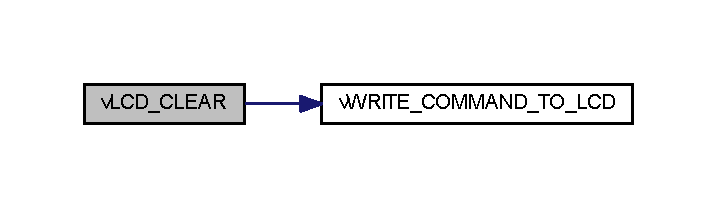
\includegraphics[width=344pt]{_lib___l_c_d_8h_a7aa490f82c8969846761762b2de7838c_cgraph}
\end{center}
\end{figure}


\hypertarget{_lib___l_c_d_8h_ad65ba27b13e2f2e52b1bf45791c42ce6}{\index{Lib\-\_\-\-L\-C\-D.\-h@{Lib\-\_\-\-L\-C\-D.\-h}!v\-L\-C\-D\-\_\-\-C\-L\-E\-A\-R\-\_\-\-B\-O\-T\-T\-O\-M@{v\-L\-C\-D\-\_\-\-C\-L\-E\-A\-R\-\_\-\-B\-O\-T\-T\-O\-M}}
\index{v\-L\-C\-D\-\_\-\-C\-L\-E\-A\-R\-\_\-\-B\-O\-T\-T\-O\-M@{v\-L\-C\-D\-\_\-\-C\-L\-E\-A\-R\-\_\-\-B\-O\-T\-T\-O\-M}!Lib_LCD.h@{Lib\-\_\-\-L\-C\-D.\-h}}
\subsubsection[{v\-L\-C\-D\-\_\-\-C\-L\-E\-A\-R\-\_\-\-B\-O\-T\-T\-O\-M}]{\setlength{\rightskip}{0pt plus 5cm}void v\-L\-C\-D\-\_\-\-C\-L\-E\-A\-R\-\_\-\-B\-O\-T\-T\-O\-M (
\begin{DoxyParamCaption}
\item[{void}]{}
\end{DoxyParamCaption}
)}}\label{_lib___l_c_d_8h_ad65ba27b13e2f2e52b1bf45791c42ce6}


Function to clear the bottom line of the L\-C\-D Display. 

Function to clear the bottom row of the display





Calls the function to set the cursor to the home position of the bottom row, write 24 spaces as a string, then return to the home position of the bottom row.

\mbox{[}in\mbox{]} nothing

\begin{DoxyReturn}{Returns}
nothing
\end{DoxyReturn}
Modification History\-:

11/17/2013 -\/ Original Function 11/24/2013 -\/ Added code to function Call function to set cursor for bottom row's home position

Call function to write string of 24 spaces to clear the bottom row

Call function to set cursor for bottom row's home position 

Definition at line 400 of file Lib\-\_\-\-L\-C\-D.\-c.


\begin{DoxyCode}
401 \{
403     \hyperlink{_lib___l_c_d_8c_ae689772c0ccc0f690d05790f3a8cd89e}{vLCD\_HOME\_BOTTOM\_LINE}();
405     \hyperlink{_lib___l_c_d_8c_a4c4dec8455090f9fa00b2c5d1fbc2543}{vLCD\_WRITE\_STRING}(\textcolor{stringliteral}{"                        "});
407     \hyperlink{_lib___l_c_d_8c_ae689772c0ccc0f690d05790f3a8cd89e}{vLCD\_HOME\_BOTTOM\_LINE}();
408 \}
\end{DoxyCode}


Here is the call graph for this function\-:\nopagebreak
\begin{figure}[H]
\begin{center}
\leavevmode
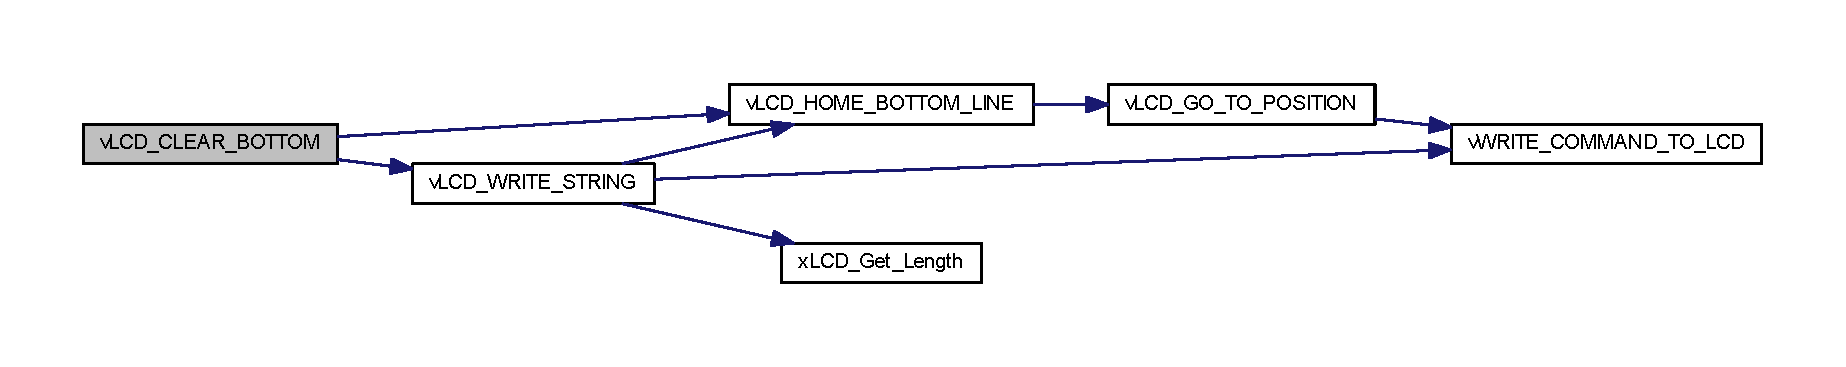
\includegraphics[width=350pt]{_lib___l_c_d_8h_ad65ba27b13e2f2e52b1bf45791c42ce6_cgraph}
\end{center}
\end{figure}


\hypertarget{_lib___l_c_d_8h_a77b96adfc0f6ba8a096e8f014885321a}{\index{Lib\-\_\-\-L\-C\-D.\-h@{Lib\-\_\-\-L\-C\-D.\-h}!v\-L\-C\-D\-\_\-\-C\-L\-E\-A\-R\-\_\-\-T\-O\-P@{v\-L\-C\-D\-\_\-\-C\-L\-E\-A\-R\-\_\-\-T\-O\-P}}
\index{v\-L\-C\-D\-\_\-\-C\-L\-E\-A\-R\-\_\-\-T\-O\-P@{v\-L\-C\-D\-\_\-\-C\-L\-E\-A\-R\-\_\-\-T\-O\-P}!Lib_LCD.h@{Lib\-\_\-\-L\-C\-D.\-h}}
\subsubsection[{v\-L\-C\-D\-\_\-\-C\-L\-E\-A\-R\-\_\-\-T\-O\-P}]{\setlength{\rightskip}{0pt plus 5cm}void v\-L\-C\-D\-\_\-\-C\-L\-E\-A\-R\-\_\-\-T\-O\-P (
\begin{DoxyParamCaption}
\item[{void}]{}
\end{DoxyParamCaption}
)}}\label{_lib___l_c_d_8h_a77b96adfc0f6ba8a096e8f014885321a}


Function to clear the top line of the L\-C\-D Display. 

Function to clear the top row of the display





Calls the function to set the cursor to the home position of the top row, write 24 spaces as a string, then return to the home position of the top row.

\mbox{[}in\mbox{]} nothing

\begin{DoxyReturn}{Returns}
nothing
\end{DoxyReturn}
Modification History\-:

11/17/2013 -\/ Original Function 11/24/2013 -\/ Added code to function Call function to set cursor for top row's home position

Call function to write string of 24 spaces to clear the top row

Call function to set cursor for top row's home position 

Definition at line 369 of file Lib\-\_\-\-L\-C\-D.\-c.


\begin{DoxyCode}
370 \{
372     \hyperlink{_lib___l_c_d_8c_a4427826e170410fece5aa9ff81f13d67}{vLCD\_HOME\_TOP\_LINE}();
374     \hyperlink{_lib___l_c_d_8c_a4c4dec8455090f9fa00b2c5d1fbc2543}{vLCD\_WRITE\_STRING}(\textcolor{stringliteral}{"                        "});
376     \hyperlink{_lib___l_c_d_8c_a4427826e170410fece5aa9ff81f13d67}{vLCD\_HOME\_TOP\_LINE}();
377 \}
\end{DoxyCode}


Here is the call graph for this function\-:\nopagebreak
\begin{figure}[H]
\begin{center}
\leavevmode
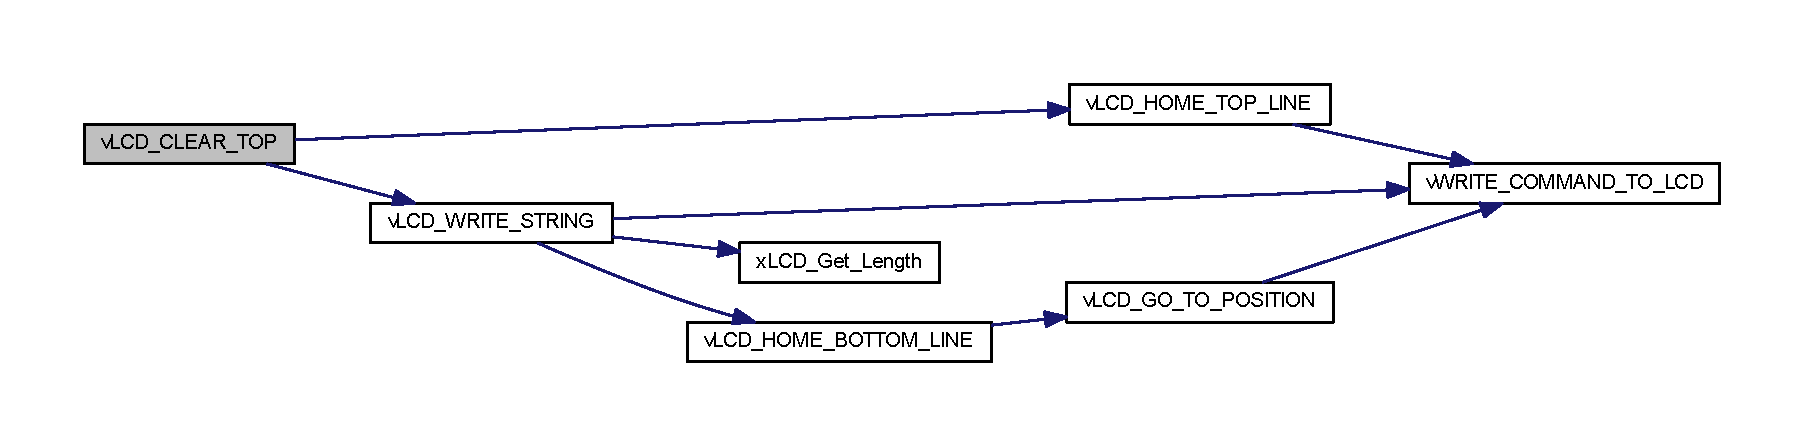
\includegraphics[width=350pt]{_lib___l_c_d_8h_a77b96adfc0f6ba8a096e8f014885321a_cgraph}
\end{center}
\end{figure}


\hypertarget{_lib___l_c_d_8h_a1c8e4b3ff3b5366283a227f3efa1b76e}{\index{Lib\-\_\-\-L\-C\-D.\-h@{Lib\-\_\-\-L\-C\-D.\-h}!v\-L\-C\-D\-\_\-\-G\-O\-\_\-\-T\-O\-\_\-\-P\-O\-S\-I\-T\-I\-O\-N@{v\-L\-C\-D\-\_\-\-G\-O\-\_\-\-T\-O\-\_\-\-P\-O\-S\-I\-T\-I\-O\-N}}
\index{v\-L\-C\-D\-\_\-\-G\-O\-\_\-\-T\-O\-\_\-\-P\-O\-S\-I\-T\-I\-O\-N@{v\-L\-C\-D\-\_\-\-G\-O\-\_\-\-T\-O\-\_\-\-P\-O\-S\-I\-T\-I\-O\-N}!Lib_LCD.h@{Lib\-\_\-\-L\-C\-D.\-h}}
\subsubsection[{v\-L\-C\-D\-\_\-\-G\-O\-\_\-\-T\-O\-\_\-\-P\-O\-S\-I\-T\-I\-O\-N}]{\setlength{\rightskip}{0pt plus 5cm}void v\-L\-C\-D\-\_\-\-G\-O\-\_\-\-T\-O\-\_\-\-P\-O\-S\-I\-T\-I\-O\-N (
\begin{DoxyParamCaption}
\item[{uint8\-\_\-t}]{, }
\item[{uint8\-\_\-t}]{}
\end{DoxyParamCaption}
)}}\label{_lib___l_c_d_8h_a1c8e4b3ff3b5366283a227f3efa1b76e}
Function To go directly to a set of X,Y coordinates on the L\-C\-D 

Definition at line 523 of file Lib\-\_\-\-L\-C\-D.\-c.


\begin{DoxyCode}
524 \{
525     \textcolor{comment}{//save the current position}
526     \textcolor{keyword}{register} uint8\_t DDRAMAddr;
527     
528     \textcolor{comment}{// For each line o the LCD}
529     \textcolor{keywordflow}{switch}(y)
530     \{
531         \textcolor{keywordflow}{case} 0: 
532             \textcolor{comment}{//for the top line, set the DDRAM address }
533             \textcolor{comment}{//move a certain number of characters to the right}
534             DDRAMAddr = LCD\_LINE0\_DDRAMADDR + x;
535         \textcolor{keywordflow}{break};
536         
537         \textcolor{keywordflow}{case} 1: 
538             \textcolor{comment}{//for the bottom line, set the DDRAM address }
539             \textcolor{comment}{//move a certain number of characters to the right}
540             DDRAMAddr = LCD\_LINE1\_DDRAMADDR + x;
541         \textcolor{keywordflow}{break};
542         
543         \textcolor{keywordflow}{default}: 
544             \textcolor{comment}{//default to the top left of the LCD if nothing is specified}
545             DDRAMAddr = LCD\_LINE0\_DDRAMADDR+x;
546     \}
547     
548     \textcolor{comment}{//save current cursor position X}
549     \hyperlink{_lib___l_c_d_8h_af3836e0e465249949a42c1711a29b026}{CURSOR\_X\_POSITION} = x;
550     \textcolor{comment}{//save current cursor position Y}
551     \hyperlink{_lib___l_c_d_8h_aa8060b8676b9666d5b1357bb896a7cfa}{CURSOR\_Y\_POSITION} = y;
552     
553     \textcolor{comment}{// send a command to set the data address}
554     \hyperlink{_lib___l_c_d_8c_a03a66d0dc99ddbf838e4699cb1f0c568}{vWRITE\_COMMAND\_TO\_LCD}(INSTR\_WR, 1 <<LCD\_DDRAM | DDRAMAddr);
555 \}
\end{DoxyCode}


Here is the call graph for this function\-:\nopagebreak
\begin{figure}[H]
\begin{center}
\leavevmode
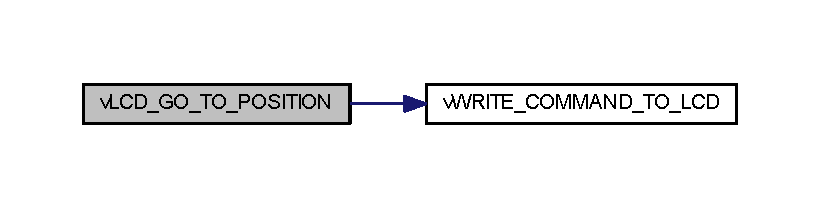
\includegraphics[width=350pt]{_lib___l_c_d_8h_a1c8e4b3ff3b5366283a227f3efa1b76e_cgraph}
\end{center}
\end{figure}




Here is the caller graph for this function\-:\nopagebreak
\begin{figure}[H]
\begin{center}
\leavevmode
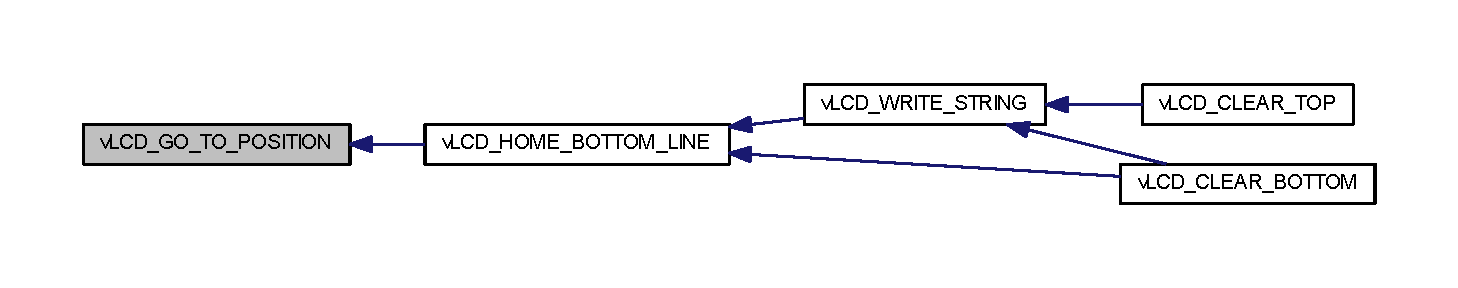
\includegraphics[width=350pt]{_lib___l_c_d_8h_a1c8e4b3ff3b5366283a227f3efa1b76e_icgraph}
\end{center}
\end{figure}


\hypertarget{_lib___l_c_d_8h_ac283786b0f4b94d35183ad4f79120bab}{\index{Lib\-\_\-\-L\-C\-D.\-h@{Lib\-\_\-\-L\-C\-D.\-h}!v\-L\-C\-D\-\_\-\-H\-O\-M\-E\-\_\-\-B\-O\-T\-T\-O\-M\-\_\-\-L\-I\-N\-E@{v\-L\-C\-D\-\_\-\-H\-O\-M\-E\-\_\-\-B\-O\-T\-T\-O\-M\-\_\-\-L\-I\-N\-E}}
\index{v\-L\-C\-D\-\_\-\-H\-O\-M\-E\-\_\-\-B\-O\-T\-T\-O\-M\-\_\-\-L\-I\-N\-E@{v\-L\-C\-D\-\_\-\-H\-O\-M\-E\-\_\-\-B\-O\-T\-T\-O\-M\-\_\-\-L\-I\-N\-E}!Lib_LCD.h@{Lib\-\_\-\-L\-C\-D.\-h}}
\subsubsection[{v\-L\-C\-D\-\_\-\-H\-O\-M\-E\-\_\-\-B\-O\-T\-T\-O\-M\-\_\-\-L\-I\-N\-E}]{\setlength{\rightskip}{0pt plus 5cm}void v\-L\-C\-D\-\_\-\-H\-O\-M\-E\-\_\-\-B\-O\-T\-T\-O\-M\-\_\-\-L\-I\-N\-E (
\begin{DoxyParamCaption}
\item[{void}]{}
\end{DoxyParamCaption}
)}}\label{_lib___l_c_d_8h_ac283786b0f4b94d35183ad4f79120bab}


Function to return to home position on the bottom line of the L\-C\-D. 

Function to go to home position on the top line of the L\-C\-D





Function is called to return the cursor to the first position on the bottom line of the L\-C\-D.

This allows for the the bottom line to be ready to write independently from the top line.

\mbox{[}in\mbox{]} none

\begin{DoxyReturn}{Returns}
nothing
\end{DoxyReturn}
Modification History\-:

11/15/2013 -\/ Original Function 

Definition at line 607 of file Lib\-\_\-\-L\-C\-D.\-c.


\begin{DoxyCode}
608 \{
609     \textcolor{comment}{//move the cursor to the bottom left position on the LCD}
610     \hyperlink{_lib___l_c_d_8c_a3d78bee51edcb0ebe6cf4936147bb207}{vLCD\_GO\_TO\_POSITION}(0,1);
611 \}
\end{DoxyCode}


Here is the call graph for this function\-:\nopagebreak
\begin{figure}[H]
\begin{center}
\leavevmode
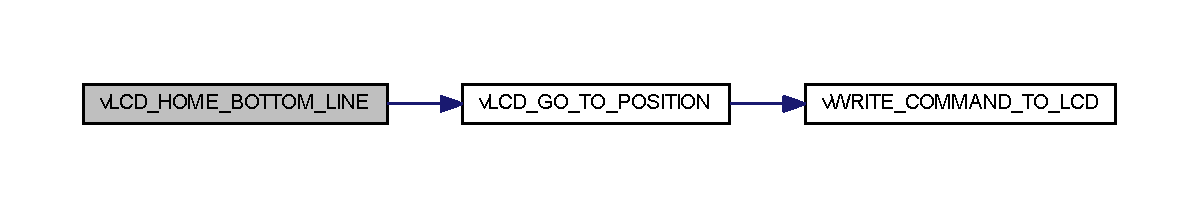
\includegraphics[width=350pt]{_lib___l_c_d_8h_ac283786b0f4b94d35183ad4f79120bab_cgraph}
\end{center}
\end{figure}




Here is the caller graph for this function\-:\nopagebreak
\begin{figure}[H]
\begin{center}
\leavevmode
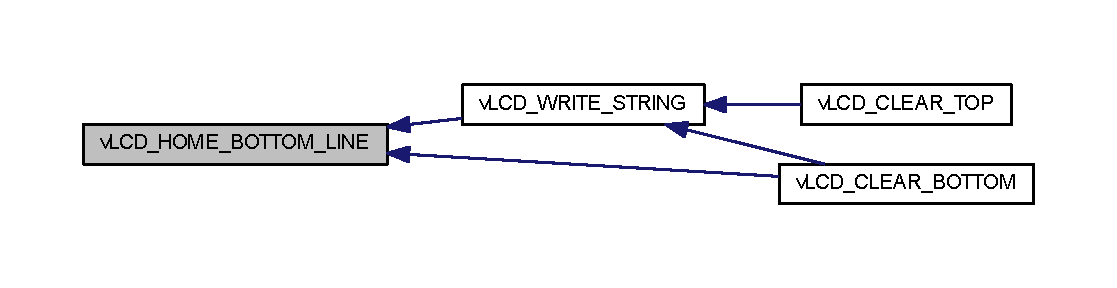
\includegraphics[width=350pt]{_lib___l_c_d_8h_ac283786b0f4b94d35183ad4f79120bab_icgraph}
\end{center}
\end{figure}


\hypertarget{_lib___l_c_d_8h_a87ae54441cf4fde7175401e8ba04c719}{\index{Lib\-\_\-\-L\-C\-D.\-h@{Lib\-\_\-\-L\-C\-D.\-h}!v\-L\-C\-D\-\_\-\-H\-O\-M\-E\-\_\-\-T\-O\-P\-\_\-\-L\-I\-N\-E@{v\-L\-C\-D\-\_\-\-H\-O\-M\-E\-\_\-\-T\-O\-P\-\_\-\-L\-I\-N\-E}}
\index{v\-L\-C\-D\-\_\-\-H\-O\-M\-E\-\_\-\-T\-O\-P\-\_\-\-L\-I\-N\-E@{v\-L\-C\-D\-\_\-\-H\-O\-M\-E\-\_\-\-T\-O\-P\-\_\-\-L\-I\-N\-E}!Lib_LCD.h@{Lib\-\_\-\-L\-C\-D.\-h}}
\subsubsection[{v\-L\-C\-D\-\_\-\-H\-O\-M\-E\-\_\-\-T\-O\-P\-\_\-\-L\-I\-N\-E}]{\setlength{\rightskip}{0pt plus 5cm}void v\-L\-C\-D\-\_\-\-H\-O\-M\-E\-\_\-\-T\-O\-P\-\_\-\-L\-I\-N\-E (
\begin{DoxyParamCaption}
\item[{void}]{}
\end{DoxyParamCaption}
)}}\label{_lib___l_c_d_8h_a87ae54441cf4fde7175401e8ba04c719}


Function to return to home position on the top line of the L\-C\-D. 

Function to go to home position on the top line of the L\-C\-D





Function is called to return the cursor to the first position on the top line of the L\-C\-D.

This allows for the the top line to be ready to write independently from the bottom line.

\mbox{[}in\mbox{]} none

\begin{DoxyReturn}{Returns}
nothing
\end{DoxyReturn}
Modification History\-:

11/15/2013 -\/ Original Function 

Definition at line 579 of file Lib\-\_\-\-L\-C\-D.\-c.


\begin{DoxyCode}
580 \{
581     \textcolor{comment}{//move cursor to the top left position of the LCD}
582     \hyperlink{_lib___l_c_d_8c_a03a66d0dc99ddbf838e4699cb1f0c568}{vWRITE\_COMMAND\_TO\_LCD}(INSTR\_WR, 1 << \hyperlink{_lib___l_c_d_8h_a207e17a2f807f034c0fc055010928a16}{LCD\_HOME\_TOP\_LINE});
583 \}
\end{DoxyCode}


Here is the call graph for this function\-:\nopagebreak
\begin{figure}[H]
\begin{center}
\leavevmode
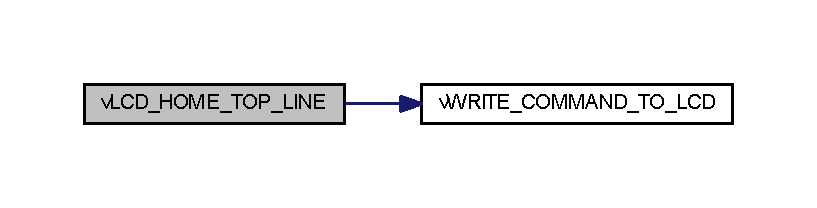
\includegraphics[width=350pt]{_lib___l_c_d_8h_a87ae54441cf4fde7175401e8ba04c719_cgraph}
\end{center}
\end{figure}




Here is the caller graph for this function\-:\nopagebreak
\begin{figure}[H]
\begin{center}
\leavevmode
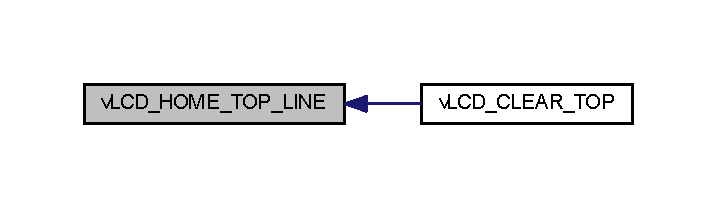
\includegraphics[width=344pt]{_lib___l_c_d_8h_a87ae54441cf4fde7175401e8ba04c719_icgraph}
\end{center}
\end{figure}


\hypertarget{_lib___l_c_d_8h_a06e60fa1f527afa2123aeb8466879f02}{\index{Lib\-\_\-\-L\-C\-D.\-h@{Lib\-\_\-\-L\-C\-D.\-h}!v\-L\-C\-D\-\_\-\-I\-N\-I\-T\-I\-A\-L\-I\-Z\-A\-T\-I\-O\-N@{v\-L\-C\-D\-\_\-\-I\-N\-I\-T\-I\-A\-L\-I\-Z\-A\-T\-I\-O\-N}}
\index{v\-L\-C\-D\-\_\-\-I\-N\-I\-T\-I\-A\-L\-I\-Z\-A\-T\-I\-O\-N@{v\-L\-C\-D\-\_\-\-I\-N\-I\-T\-I\-A\-L\-I\-Z\-A\-T\-I\-O\-N}!Lib_LCD.h@{Lib\-\_\-\-L\-C\-D.\-h}}
\subsubsection[{v\-L\-C\-D\-\_\-\-I\-N\-I\-T\-I\-A\-L\-I\-Z\-A\-T\-I\-O\-N}]{\setlength{\rightskip}{0pt plus 5cm}void v\-L\-C\-D\-\_\-\-I\-N\-I\-T\-I\-A\-L\-I\-Z\-A\-T\-I\-O\-N (
\begin{DoxyParamCaption}
\item[{void}]{}
\end{DoxyParamCaption}
)}}\label{_lib___l_c_d_8h_a06e60fa1f527afa2123aeb8466879f02}


Function to initialize the L\-D\-C. 

Function to Initialize an L\-C\-D Display





Function is called to initialize the L\-C\-D into either 4 bit or 8 bit mode off of the flowcharts on pages 26 and 27 of the K\-S6600\-U datasheet

\mbox{[}in\mbox{]} none

\begin{DoxyReturn}{Returns}
nothing
\end{DoxyReturn}
Modification History\-:

11/17/2013 -\/ Original Function 

Definition at line 48 of file Lib\-\_\-\-L\-C\-D.\-c.


\begin{DoxyCode}
49 \{
50     \textcolor{keywordtype}{unsigned} \textcolor{keywordtype}{char} Instructions = 0x00;
51     
52 \textcolor{preprocessor}{    #ifdef BITMODE4}
53 \textcolor{preprocessor}{}
54         \_delay\_ms(35);
55         
56         \textcolor{comment}{/***************************************************************************/}
65         Instructions = (1<<\hyperlink{_lib___l_c_d_8h_a5b91fe480c768d4f246f3890207bfbfc}{LCD\_D5});
66         
67         \hyperlink{_lib___l_c_d_8c_a03a66d0dc99ddbf838e4699cb1f0c568}{vWRITE\_COMMAND\_TO\_LCD}(INSTR\_WR, Instructions);
68         \hyperlink{_lib___l_c_d_8c_a03a66d0dc99ddbf838e4699cb1f0c568}{vWRITE\_COMMAND\_TO\_LCD}(INSTR\_WR, Instructions);
69         
70         Instructions = (TWO\_LINE\_MODE<<\hyperlink{_lib___l_c_d_8h_abd65075e01c7413419581aedee5bcc24}{LCD\_D7})|(DISPLAY\_ON<<\hyperlink{_lib___l_c_d_8h_a72e105fcda5fd1c07b5f391379a439d4}{LCD\_D6});
71         
72         \hyperlink{_lib___l_c_d_8c_a03a66d0dc99ddbf838e4699cb1f0c568}{vWRITE\_COMMAND\_TO\_LCD}(INSTR\_WR, Instructions);
73         
75         \_delay\_us(50);
76         
77         \textcolor{comment}{/***************************************************************************/}
87         Instructions = 0x00;
88         
89         \hyperlink{_lib___l_c_d_8c_a03a66d0dc99ddbf838e4699cb1f0c568}{vWRITE\_COMMAND\_TO\_LCD}(INSTR\_WR, Instructions);
90         
91         Instructions = (1 << \hyperlink{_lib___l_c_d_8h_abd65075e01c7413419581aedee5bcc24}{LCD\_D7}) | 
92               (DISPLAY\_ON << \hyperlink{_lib___l_c_d_8h_a72e105fcda5fd1c07b5f391379a439d4}{LCD\_D6}) | 
93                (CURSOR\_ON << \hyperlink{_lib___l_c_d_8h_a5b91fe480c768d4f246f3890207bfbfc}{LCD\_D5}) | 
94          (CURSOR\_BLINK\_ON << \hyperlink{_lib___l_c_d_8h_ade7e247311032a474711416da480ed8b}{LCD\_D4}));
95          
96          \hyperlink{_lib___l_c_d_8c_a03a66d0dc99ddbf838e4699cb1f0c568}{vWRITE\_COMMAND\_TO\_LCD}(INSTR\_WR, Instructions);
97          
99         \_delay\_us(50);
100         
101         \textcolor{comment}{/***************************************************************************/}
105         Instructions = 0x00;
106         
107         \hyperlink{_lib___l_c_d_8c_a03a66d0dc99ddbf838e4699cb1f0c568}{vWRITE\_COMMAND\_TO\_LCD}(INSTR\_WR, Instructions);
108         
111         Instructions = (1<<\hyperlink{_lib___l_c_d_8h_ade7e247311032a474711416da480ed8b}{LCD\_D4});
112         
113         \hyperlink{_lib___l_c_d_8c_a03a66d0dc99ddbf838e4699cb1f0c568}{vWRITE\_COMMAND\_TO\_LCD}(INSTR\_WR, Instructions);
114         
116         \_delay\_us(1600);
117         
118         \textcolor{comment}{/***************************************************************************/}
122         Instructions = 0x00;
123         
124         \hyperlink{_lib___l_c_d_8c_a03a66d0dc99ddbf838e4699cb1f0c568}{vWRITE\_COMMAND\_TO\_LCD}(INSTR\_WR, Instructions);
125         
131         Instructions =  (1 << \hyperlink{_lib___l_c_d_8h_a72e105fcda5fd1c07b5f391379a439d4}{LCD\_D6}) | 
132            (INCREMENT\_MODE << \hyperlink{_lib___l_c_d_8h_a5b91fe480c768d4f246f3890207bfbfc}{LCD\_D5}) | 
133         (ENTIRE\_SHIFT\_MODE << \hyperlink{_lib___l_c_d_8h_ade7e247311032a474711416da480ed8b}{LCD\_D4});
134         
135         \hyperlink{_lib___l_c_d_8c_a03a66d0dc99ddbf838e4699cb1f0c568}{vWRITE\_COMMAND\_TO\_LCD}(INSTR\_WR, Instructions);
136 \textcolor{preprocessor}{    #endif;}
137 \textcolor{preprocessor}{}    
138 \textcolor{preprocessor}{    #ifdef BITMODE8}
139 \textcolor{preprocessor}{}    
141         \_delay\_ms(35);
142         
143         \textcolor{comment}{/***************************************************************************/}
152         Instructions = (1 << \hyperlink{_lib___l_c_d_8h_a5b91fe480c768d4f246f3890207bfbfc}{LCD\_D5}) |
153                        (1 << \hyperlink{_lib___l_c_d_8h_ade7e247311032a474711416da480ed8b}{LCD\_D4}) | 
154            (TWO\_LINE\_MODE << \hyperlink{_lib___l_c_d_8h_a3d23f1f20ad1f0fb190f4a10334f4bf1}{LCD\_D3}) | 
155               (DISPLAY\_ON << \hyperlink{_lib___l_c_d_8h_aa97ea257a9007a9055e5f77e1b3336e5}{LCD\_D2}); 
156               
157         \hyperlink{_lib___l_c_d_8c_a03a66d0dc99ddbf838e4699cb1f0c568}{vWRITE\_COMMAND\_TO\_LCD}(INSTR\_WR, Instructions);
158                 
160         \_delay\_us(50);
161         
162         \textcolor{comment}{/***************************************************************************/}
172         Instructions = (1 << \hyperlink{_lib___l_c_d_8h_a3d23f1f20ad1f0fb190f4a10334f4bf1}{LCD\_D3}) | 
173               (DISPLAY\_ON << \hyperlink{_lib___l_c_d_8h_aa97ea257a9007a9055e5f77e1b3336e5}{LCD\_D2}) | 
174                (CURSOR\_ON << \hyperlink{_lib___l_c_d_8h_ac6b74016e58d58b47230a2d0aaf959d8}{LCD\_D1}) | 
175          (CURSOR\_BLINK\_ON << 0);
176          
177          \hyperlink{_lib___l_c_d_8c_a03a66d0dc99ddbf838e4699cb1f0c568}{vWRITE\_COMMAND\_TO\_LCD}(INSTR\_WR, Instructions);
178          
180         \_delay\_us(50);
181         
182         \textcolor{comment}{/***************************************************************************/}
188         Instructions = 0x01;
189         
190         \hyperlink{_lib___l_c_d_8c_a03a66d0dc99ddbf838e4699cb1f0c568}{vWRITE\_COMMAND\_TO\_LCD}(INSTR\_WR, Instructions);
191         
193         \_delay\_us(1600);
194         
195         \textcolor{comment}{/***************************************************************************/}
204         Instructions =  (1 << \hyperlink{_lib___l_c_d_8h_aa97ea257a9007a9055e5f77e1b3336e5}{LCD\_D2}) | 
205            (INCREMENT\_MODE << \hyperlink{_lib___l_c_d_8h_ac6b74016e58d58b47230a2d0aaf959d8}{LCD\_D1}) | 
206         (ENTIRE\_SHIFT\_MODE << 0);
207         
208         \hyperlink{_lib___l_c_d_8c_a03a66d0dc99ddbf838e4699cb1f0c568}{vWRITE\_COMMAND\_TO\_LCD}(INSTR\_WR, Instructions);
209         
210 \textcolor{preprocessor}{    #endif;}
211 \textcolor{preprocessor}{}    
212 \}
\end{DoxyCode}


Here is the call graph for this function\-:\nopagebreak
\begin{figure}[H]
\begin{center}
\leavevmode
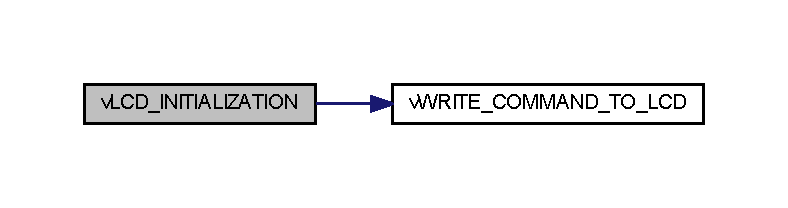
\includegraphics[width=350pt]{_lib___l_c_d_8h_a06e60fa1f527afa2123aeb8466879f02_cgraph}
\end{center}
\end{figure}


\hypertarget{_lib___l_c_d_8h_aa045d5303123d31b306dbd38aa476da2}{\index{Lib\-\_\-\-L\-C\-D.\-h@{Lib\-\_\-\-L\-C\-D.\-h}!v\-L\-C\-D\-\_\-\-O\-N\-\_\-\-O\-F\-F@{v\-L\-C\-D\-\_\-\-O\-N\-\_\-\-O\-F\-F}}
\index{v\-L\-C\-D\-\_\-\-O\-N\-\_\-\-O\-F\-F@{v\-L\-C\-D\-\_\-\-O\-N\-\_\-\-O\-F\-F}!Lib_LCD.h@{Lib\-\_\-\-L\-C\-D.\-h}}
\subsubsection[{v\-L\-C\-D\-\_\-\-O\-N\-\_\-\-O\-F\-F}]{\setlength{\rightskip}{0pt plus 5cm}void v\-L\-C\-D\-\_\-\-O\-N\-\_\-\-O\-F\-F (
\begin{DoxyParamCaption}
\item[{void}]{}
\end{DoxyParamCaption}
)}}\label{_lib___l_c_d_8h_aa045d5303123d31b306dbd38aa476da2}


Function to toggle L\-C\-D on and off. 

Toggles L\-C\-D Display on and off





Checks the current status of the L\-C\-D. If the L\-C\-D is on, toggle it so it's off. If the L\-C\-D is off, turn it on. Uses the v\-L\-C\-D\-\_\-\-W\-R\-I\-T\-E command to send instructions to the L\-C\-D.

\mbox{[}in\mbox{]} nothing

\begin{DoxyReturn}{Returns}
nothing
\end{DoxyReturn}
Modification History\-:

11/18/2013 -\/ Original Function 11/24/2013 -\/ Added code to function Create command to toggle L\-C\-D Display

Toggle the On\-Off\-Status tracker variable

Toggle L\-C\-D 

Definition at line 431 of file Lib\-\_\-\-L\-C\-D.\-c.


\begin{DoxyCode}
432 \{
434     uint8\_t LCD\_Command = 
435         (1 << \hyperlink{_lib___l_c_d_8h_aa57a26c661193bfb41377f080d15b4d6}{LCD\_ON\_OFF\_INSTRCUTION}) |
436         (\hyperlink{_lib___l_c_d_8h_a7306354fa1b76399437e38800816c915}{OnOffStatus} << LCD\_ON\_INSTRUCTION) |
437         (\hyperlink{_lib___l_c_d_8h_aaa9d50b1d874e351a1bafc33f7f8b22d}{configCURSOR\_SHOW} << LCD\_CURSOR\_SHOW\_INSTRUCTION) |
438         (configCURSOR\_BLINK << LCD\_CURSOR\_BLINK\_INSTRUCTION);
439     
441     \hyperlink{_lib___l_c_d_8h_a7306354fa1b76399437e38800816c915}{OnOffStatus} = \hyperlink{_lib___l_c_d_8h_a7306354fa1b76399437e38800816c915}{OnOffStatus} ^ 0x01;
442     
444     \hyperlink{_lib___l_c_d_8c_a03a66d0dc99ddbf838e4699cb1f0c568}{vWRITE\_COMMAND\_TO\_LCD}(0, LCD\_Command);
445 \}
\end{DoxyCode}


Here is the call graph for this function\-:\nopagebreak
\begin{figure}[H]
\begin{center}
\leavevmode
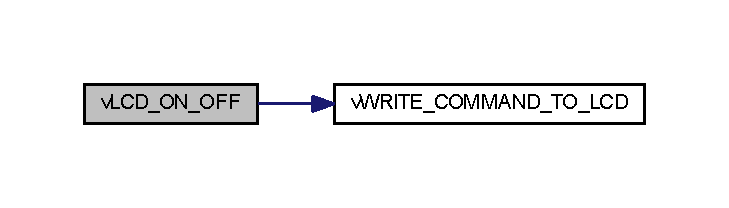
\includegraphics[width=350pt]{_lib___l_c_d_8h_aa045d5303123d31b306dbd38aa476da2_cgraph}
\end{center}
\end{figure}


\hypertarget{_lib___l_c_d_8h_ab1a34cbfaa919c3fd0ef3804929ae75e}{\index{Lib\-\_\-\-L\-C\-D.\-h@{Lib\-\_\-\-L\-C\-D.\-h}!v\-L\-C\-D\-\_\-\-W\-R\-I\-T\-E\-\_\-\-S\-T\-R\-I\-N\-G@{v\-L\-C\-D\-\_\-\-W\-R\-I\-T\-E\-\_\-\-S\-T\-R\-I\-N\-G}}
\index{v\-L\-C\-D\-\_\-\-W\-R\-I\-T\-E\-\_\-\-S\-T\-R\-I\-N\-G@{v\-L\-C\-D\-\_\-\-W\-R\-I\-T\-E\-\_\-\-S\-T\-R\-I\-N\-G}!Lib_LCD.h@{Lib\-\_\-\-L\-C\-D.\-h}}
\subsubsection[{v\-L\-C\-D\-\_\-\-W\-R\-I\-T\-E\-\_\-\-S\-T\-R\-I\-N\-G}]{\setlength{\rightskip}{0pt plus 5cm}void v\-L\-C\-D\-\_\-\-W\-R\-I\-T\-E\-\_\-\-S\-T\-R\-I\-N\-G (
\begin{DoxyParamCaption}
\item[{char $\ast$}]{str\-\_\-ptr}
\end{DoxyParamCaption}
)}}\label{_lib___l_c_d_8h_ab1a34cbfaa919c3fd0ef3804929ae75e}


Function to write strings to the L\-C\-D. 

Functions to write strings to an L\-C\-D





Function is used to take in a string of characters and display the string to the L\-C\-D

\mbox{[}in\mbox{]} $\ast$str\-\_\-ptr

\begin{DoxyReturn}{Returns}
nothing
\end{DoxyReturn}
Modification History\-:

11/17/2013 -\/ Original Function 11/23/2013 -\/ Addec Code If text wrap is enabled 

Definition at line 295 of file Lib\-\_\-\-L\-C\-D.\-c.


\begin{DoxyCode}
296 \{   
297     \textcolor{keywordflow}{while}(*str\_ptr != \textcolor{charliteral}{'\(\backslash\)0'})     \textcolor{comment}{//move through the string until the end is reached}
298     \{
300 \textcolor{preprocessor}{        #ifdef configTEXT\_WRAP}
301 \textcolor{preprocessor}{}\textcolor{preprocessor}{            #if configTEXT\_WRAP == 1}
302 \textcolor{preprocessor}{}        
304                 \textcolor{keywordflow}{if}( \hyperlink{_lib___l_c_d_8c_a1d0d7788aeded6a84e4149f2351beaf8}{xLCD\_Get\_Length}()== 24)
305                     \hyperlink{_lib___l_c_d_8c_ae689772c0ccc0f690d05790f3a8cd89e}{vLCD\_HOME\_BOTTOM\_LINE}(); \textcolor{comment}{//Continue on to the bottom line}
306         
307 \textcolor{preprocessor}{            #endif}
308 \textcolor{preprocessor}{}\textcolor{preprocessor}{        #endif}
309 \textcolor{preprocessor}{}        \hyperlink{_lib___l_c_d_8c_a03a66d0dc99ddbf838e4699cb1f0c568}{vWRITE\_COMMAND\_TO\_LCD}(DATA\_WR, *str\_ptr++);
310     \}   
311 \}
\end{DoxyCode}


Here is the call graph for this function\-:\nopagebreak
\begin{figure}[H]
\begin{center}
\leavevmode
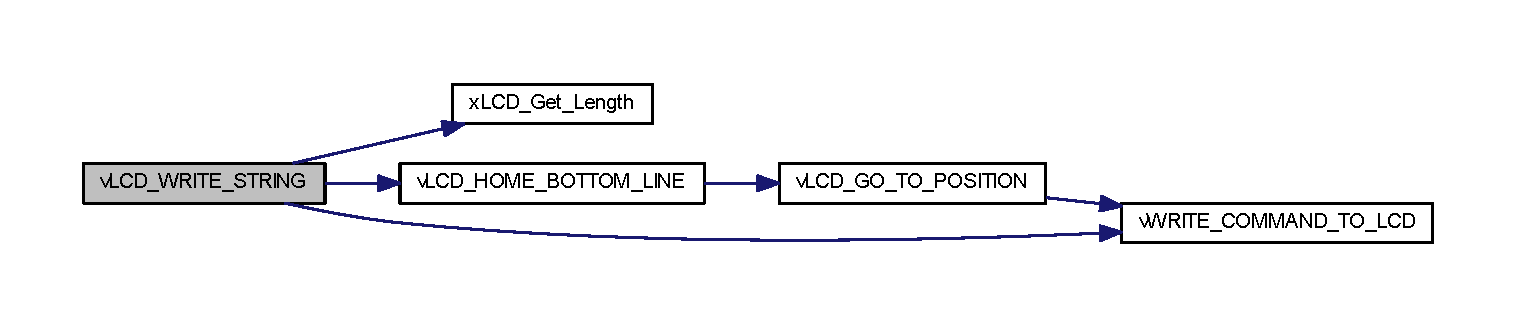
\includegraphics[width=350pt]{_lib___l_c_d_8h_ab1a34cbfaa919c3fd0ef3804929ae75e_cgraph}
\end{center}
\end{figure}




Here is the caller graph for this function\-:\nopagebreak
\begin{figure}[H]
\begin{center}
\leavevmode
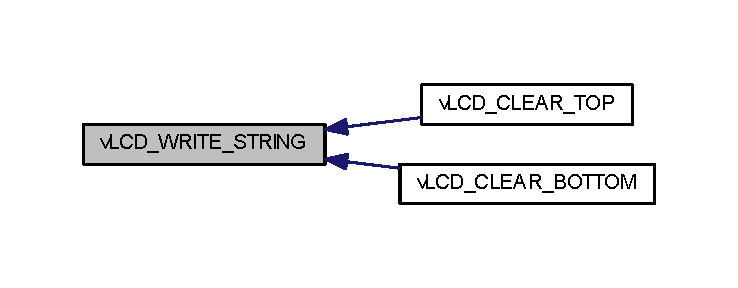
\includegraphics[width=350pt]{_lib___l_c_d_8h_ab1a34cbfaa919c3fd0ef3804929ae75e_icgraph}
\end{center}
\end{figure}


\hypertarget{_lib___l_c_d_8h_a03a66d0dc99ddbf838e4699cb1f0c568}{\index{Lib\-\_\-\-L\-C\-D.\-h@{Lib\-\_\-\-L\-C\-D.\-h}!v\-W\-R\-I\-T\-E\-\_\-\-C\-O\-M\-M\-A\-N\-D\-\_\-\-T\-O\-\_\-\-L\-C\-D@{v\-W\-R\-I\-T\-E\-\_\-\-C\-O\-M\-M\-A\-N\-D\-\_\-\-T\-O\-\_\-\-L\-C\-D}}
\index{v\-W\-R\-I\-T\-E\-\_\-\-C\-O\-M\-M\-A\-N\-D\-\_\-\-T\-O\-\_\-\-L\-C\-D@{v\-W\-R\-I\-T\-E\-\_\-\-C\-O\-M\-M\-A\-N\-D\-\_\-\-T\-O\-\_\-\-L\-C\-D}!Lib_LCD.h@{Lib\-\_\-\-L\-C\-D.\-h}}
\subsubsection[{v\-W\-R\-I\-T\-E\-\_\-\-C\-O\-M\-M\-A\-N\-D\-\_\-\-T\-O\-\_\-\-L\-C\-D}]{\setlength{\rightskip}{0pt plus 5cm}void v\-W\-R\-I\-T\-E\-\_\-\-C\-O\-M\-M\-A\-N\-D\-\_\-\-T\-O\-\_\-\-L\-C\-D (
\begin{DoxyParamCaption}
\item[{char}]{R\-S, }
\item[{char}]{data}
\end{DoxyParamCaption}
)}}\label{_lib___l_c_d_8h_a03a66d0dc99ddbf838e4699cb1f0c568}
Function to Write commands to an L\-C\-D Set Read/\-Write High

Set D\-B7 pin to read

Wait for Busy flag to clear

Set L\-C\-D\-\_\-\-D7 pin for output

Enable display for use

Wait for Busy flag to clear 

Definition at line 238 of file Lib\-\_\-\-L\-C\-D.\-c.


\begin{DoxyCode}
239 \{
240     \textcolor{keywordflow}{if}(RS == DATA\_WR) \hyperlink{_lib___l_c_d_8h_a488115f911c9dcfb0bad83c6b0912965}{LCP} = 1<<\hyperlink{_lib___l_c_d_8h_a4781e073871c6f27f89b9463ad3a4ed1}{LCD\_RS}; \textcolor{comment}{/*Set RS high to write data*/} 
241     \textcolor{keywordflow}{else} \hyperlink{_lib___l_c_d_8h_a488115f911c9dcfb0bad83c6b0912965}{LCP} = 0x00; \textcolor{comment}{/*Set RS low to write instructions*/}
242     
244     \hyperlink{_lib___l_c_d_8h_a488115f911c9dcfb0bad83c6b0912965}{LCP} = \hyperlink{_lib___l_c_d_8h_a488115f911c9dcfb0bad83c6b0912965}{LCP} | 1<<\hyperlink{_lib___l_c_d_8h_a26089a10ddd59a0dc7283c19ccc02533}{LCD\_RW}; 
245 
247     \hyperlink{_lib___l_c_d_8h_a8a47e7956b4dd0e990db51cd70d9eac8}{LDDR} = \hyperlink{_lib___l_c_d_8h_a8a47e7956b4dd0e990db51cd70d9eac8}{LDDR} & 0x7F;
248     
250     \textcolor{keywordflow}{while}(\hyperlink{_lib___l_c_d_8h_a88979bbbc6cd7d8c557867826d755c1b}{LDP} & 0x80);
251     
253     \hyperlink{_lib___l_c_d_8h_a8a47e7956b4dd0e990db51cd70d9eac8}{LDDR} = \hyperlink{_lib___l_c_d_8h_a8a47e7956b4dd0e990db51cd70d9eac8}{LDDR} | (1 << \hyperlink{_lib___l_c_d_8h_abd65075e01c7413419581aedee5bcc24}{LCD\_D7});
254     
255     \textcolor{keywordflow}{if}(RS == DATA\_WR) \hyperlink{_lib___l_c_d_8h_a488115f911c9dcfb0bad83c6b0912965}{LCP} = 1 << \hyperlink{_lib___l_c_d_8h_a4781e073871c6f27f89b9463ad3a4ed1}{LCD\_RS};   \textcolor{comment}{/*Set RS high to write data*/} 
256     \textcolor{keywordflow}{else} \hyperlink{_lib___l_c_d_8h_a488115f911c9dcfb0bad83c6b0912965}{LCP} = 0x00; \textcolor{comment}{/*Set RS low to write instructions*/}
257     
259     \hyperlink{_lib___l_c_d_8h_a488115f911c9dcfb0bad83c6b0912965}{LCP} = \hyperlink{_lib___l_c_d_8h_a488115f911c9dcfb0bad83c6b0912965}{LCP} | 1<<\hyperlink{_lib___l_c_d_8h_a6ec15b1e813d1f56d2eb644a127e5d49}{LCD\_E}; 
260     
261     \textcolor{comment}{/* Write Data*/}
262     \hyperlink{_lib___l_c_d_8h_a88979bbbc6cd7d8c557867826d755c1b}{LDP} = data;
263     
265     \textcolor{keywordflow}{while}(\hyperlink{_lib___l_c_d_8h_a88979bbbc6cd7d8c557867826d755c1b}{LDP} & 0x80); 
266     
267     \textcolor{comment}{/*Set Read/Write low*/}
268     \hyperlink{_lib___l_c_d_8h_a488115f911c9dcfb0bad83c6b0912965}{LCP} = \hyperlink{_lib___l_c_d_8h_a488115f911c9dcfb0bad83c6b0912965}{LCP} & 1<<\hyperlink{_lib___l_c_d_8h_a4781e073871c6f27f89b9463ad3a4ed1}{LCD\_RS};
269     
270     \textcolor{comment}{/*Delay for at least 50us*/}
271     \_delay\_us(50);
272 \}
\end{DoxyCode}


Here is the caller graph for this function\-:\nopagebreak
\begin{figure}[H]
\begin{center}
\leavevmode
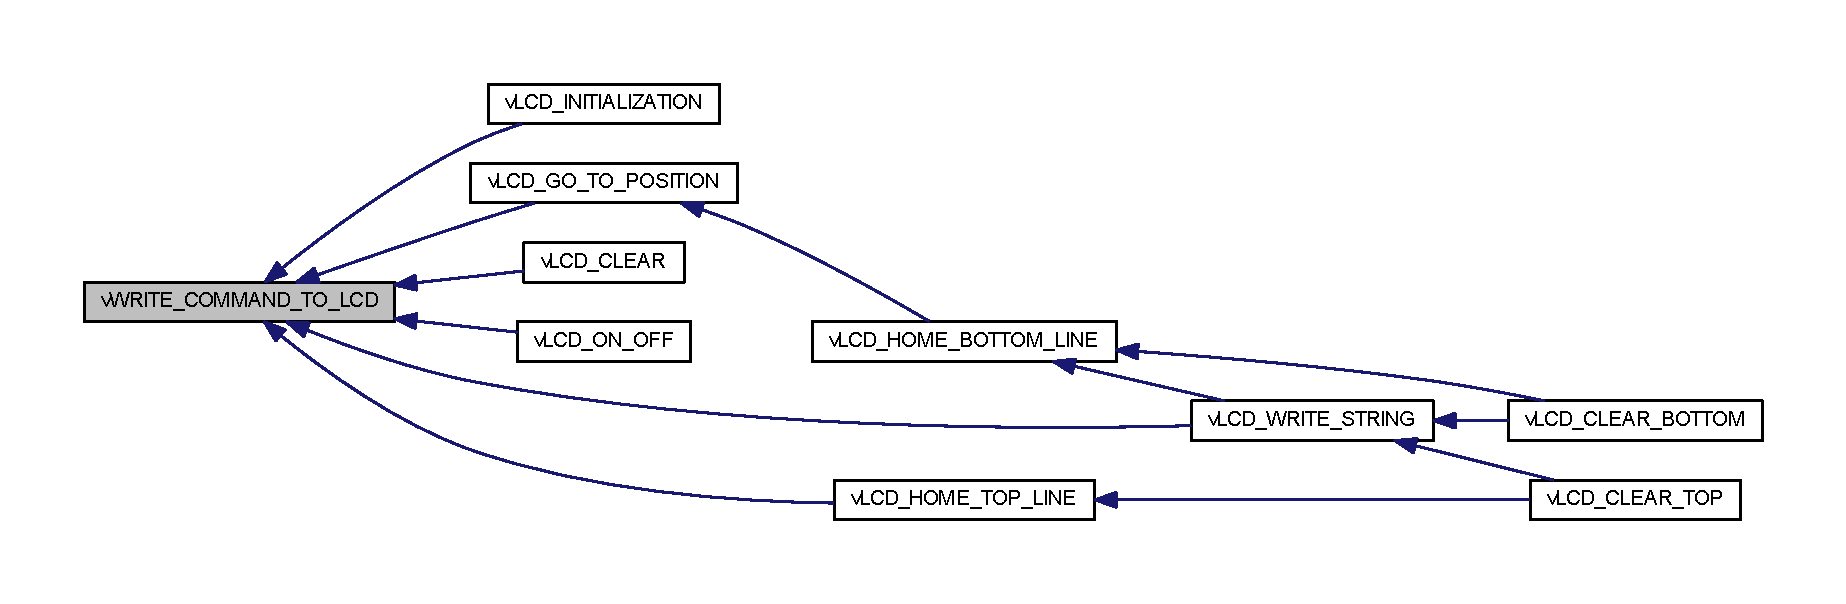
\includegraphics[width=350pt]{_lib___l_c_d_8h_a03a66d0dc99ddbf838e4699cb1f0c568_icgraph}
\end{center}
\end{figure}


\hypertarget{_lib___l_c_d_8h_ada06c4c8d18a84974788d6a726439302}{\index{Lib\-\_\-\-L\-C\-D.\-h@{Lib\-\_\-\-L\-C\-D.\-h}!x\-L\-C\-D\-\_\-\-Get\-\_\-\-Length@{x\-L\-C\-D\-\_\-\-Get\-\_\-\-Length}}
\index{x\-L\-C\-D\-\_\-\-Get\-\_\-\-Length@{x\-L\-C\-D\-\_\-\-Get\-\_\-\-Length}!Lib_LCD.h@{Lib\-\_\-\-L\-C\-D.\-h}}
\subsubsection[{x\-L\-C\-D\-\_\-\-Get\-\_\-\-Length}]{\setlength{\rightskip}{0pt plus 5cm}uint8\-\_\-t x\-L\-C\-D\-\_\-\-Get\-\_\-\-Length (
\begin{DoxyParamCaption}
{}
\end{DoxyParamCaption}
)}}\label{_lib___l_c_d_8h_ada06c4c8d18a84974788d6a726439302}
Function to track remaining characters on the L\-C\-D If the cursor is on the top line

give total available characters(top and bottom line)

If the cursor is on the bottom line

Give remaining characters available. 

Definition at line 475 of file Lib\-\_\-\-L\-C\-D.\-c.


\begin{DoxyCode}
476 \{
477     \textcolor{keywordflow}{switch}(\hyperlink{_lib___l_c_d_8h_aa8060b8676b9666d5b1357bb896a7cfa}{CURSOR\_Y\_POSITION})
478     \{
480         \textcolor{keywordflow}{case} 0:
482             \textcolor{keywordflow}{return} 48 - \hyperlink{_lib___l_c_d_8h_af3836e0e465249949a42c1711a29b026}{CURSOR\_X\_POSITION}; 
483             \textcolor{keywordflow}{break};
484             
486         \textcolor{keywordflow}{case} 1:
488             \textcolor{keywordflow}{return} 24 - \hyperlink{_lib___l_c_d_8h_af3836e0e465249949a42c1711a29b026}{CURSOR\_X\_POSITION}; 
489     \}
490 \}
\end{DoxyCode}


Here is the caller graph for this function\-:\nopagebreak
\begin{figure}[H]
\begin{center}
\leavevmode
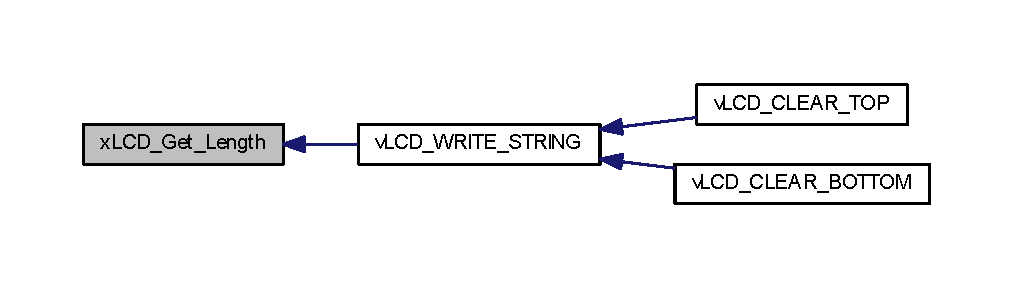
\includegraphics[width=350pt]{_lib___l_c_d_8h_ada06c4c8d18a84974788d6a726439302_icgraph}
\end{center}
\end{figure}




\subsection{Variable Documentation}
\hypertarget{_lib___l_c_d_8h_a2a0ae8d2213f4ce1b8aa972992adf1c3}{\index{Lib\-\_\-\-L\-C\-D.\-h@{Lib\-\_\-\-L\-C\-D.\-h}!Bottom\-Length@{Bottom\-Length}}
\index{Bottom\-Length@{Bottom\-Length}!Lib_LCD.h@{Lib\-\_\-\-L\-C\-D.\-h}}
\subsubsection[{Bottom\-Length}]{\setlength{\rightskip}{0pt plus 5cm}uint8\-\_\-t Bottom\-Length}}\label{_lib___l_c_d_8h_a2a0ae8d2213f4ce1b8aa972992adf1c3}
Variable to track the characters used on the bottom line of the L\-C\-D 

Definition at line 31 of file Lib\-\_\-\-L\-C\-D.\-h.

\hypertarget{_lib___l_c_d_8h_af3836e0e465249949a42c1711a29b026}{\index{Lib\-\_\-\-L\-C\-D.\-h@{Lib\-\_\-\-L\-C\-D.\-h}!C\-U\-R\-S\-O\-R\-\_\-\-X\-\_\-\-P\-O\-S\-I\-T\-I\-O\-N@{C\-U\-R\-S\-O\-R\-\_\-\-X\-\_\-\-P\-O\-S\-I\-T\-I\-O\-N}}
\index{C\-U\-R\-S\-O\-R\-\_\-\-X\-\_\-\-P\-O\-S\-I\-T\-I\-O\-N@{C\-U\-R\-S\-O\-R\-\_\-\-X\-\_\-\-P\-O\-S\-I\-T\-I\-O\-N}!Lib_LCD.h@{Lib\-\_\-\-L\-C\-D.\-h}}
\subsubsection[{C\-U\-R\-S\-O\-R\-\_\-\-X\-\_\-\-P\-O\-S\-I\-T\-I\-O\-N}]{\setlength{\rightskip}{0pt plus 5cm}uint8\-\_\-t C\-U\-R\-S\-O\-R\-\_\-\-X\-\_\-\-P\-O\-S\-I\-T\-I\-O\-N}}\label{_lib___l_c_d_8h_af3836e0e465249949a42c1711a29b026}
Variable to track the cursor character position 

Definition at line 43 of file Lib\-\_\-\-L\-C\-D.\-h.

\hypertarget{_lib___l_c_d_8h_aa8060b8676b9666d5b1357bb896a7cfa}{\index{Lib\-\_\-\-L\-C\-D.\-h@{Lib\-\_\-\-L\-C\-D.\-h}!C\-U\-R\-S\-O\-R\-\_\-\-Y\-\_\-\-P\-O\-S\-I\-T\-I\-O\-N@{C\-U\-R\-S\-O\-R\-\_\-\-Y\-\_\-\-P\-O\-S\-I\-T\-I\-O\-N}}
\index{C\-U\-R\-S\-O\-R\-\_\-\-Y\-\_\-\-P\-O\-S\-I\-T\-I\-O\-N@{C\-U\-R\-S\-O\-R\-\_\-\-Y\-\_\-\-P\-O\-S\-I\-T\-I\-O\-N}!Lib_LCD.h@{Lib\-\_\-\-L\-C\-D.\-h}}
\subsubsection[{C\-U\-R\-S\-O\-R\-\_\-\-Y\-\_\-\-P\-O\-S\-I\-T\-I\-O\-N}]{\setlength{\rightskip}{0pt plus 5cm}uint8\-\_\-t C\-U\-R\-S\-O\-R\-\_\-\-Y\-\_\-\-P\-O\-S\-I\-T\-I\-O\-N}}\label{_lib___l_c_d_8h_aa8060b8676b9666d5b1357bb896a7cfa}
Variable to track the line that the cursor is on 

Definition at line 45 of file Lib\-\_\-\-L\-C\-D.\-h.

\hypertarget{_lib___l_c_d_8h_a7306354fa1b76399437e38800816c915}{\index{Lib\-\_\-\-L\-C\-D.\-h@{Lib\-\_\-\-L\-C\-D.\-h}!On\-Off\-Status@{On\-Off\-Status}}
\index{On\-Off\-Status@{On\-Off\-Status}!Lib_LCD.h@{Lib\-\_\-\-L\-C\-D.\-h}}
\subsubsection[{On\-Off\-Status}]{\setlength{\rightskip}{0pt plus 5cm}uint8\-\_\-t On\-Off\-Status = 0}}\label{_lib___l_c_d_8h_a7306354fa1b76399437e38800816c915}
Variable to track the on/off status of the L\-C\-D 0-\/off 1-\/on  Zero is off 

Definition at line 58 of file Lib\-\_\-\-L\-C\-D.\-h.

\hypertarget{_lib___l_c_d_8h_a73f11c737d331ba1fff0e24bf7169ca1}{\index{Lib\-\_\-\-L\-C\-D.\-h@{Lib\-\_\-\-L\-C\-D.\-h}!Top\-\_\-\-Length@{Top\-\_\-\-Length}}
\index{Top\-\_\-\-Length@{Top\-\_\-\-Length}!Lib_LCD.h@{Lib\-\_\-\-L\-C\-D.\-h}}
\subsubsection[{Top\-\_\-\-Length}]{\setlength{\rightskip}{0pt plus 5cm}uint8\-\_\-t Top\-\_\-\-Length}}\label{_lib___l_c_d_8h_a73f11c737d331ba1fff0e24bf7169ca1}
Variable to track the characters used on the top line of the L\-C\-D 

Definition at line 33 of file Lib\-\_\-\-L\-C\-D.\-h.


%--- End generated contents ---

% Index
\newpage
\phantomsection
\addcontentsline{toc}{part}{Index}
\printindex

\end{document}
